\documentclass[12pt]{iopart}
%DIF LATEXDIFF DIFFERENCE FILE
%DIF DEL submission_01.tex   Fri Apr 23 09:06:12 2021
%DIF ADD submission_02.tex   Tue May  4 21:46:09 2021

\usepackage{graphicx}
\graphicspath{{../fig/}}

\usepackage{url}
\usepackage{siunitx}
\usepackage{cleveref}
%DIF PREAMBLE EXTENSION ADDED BY LATEXDIFF
%DIF UNDERLINE PREAMBLE %DIF PREAMBLE
\RequirePackage[normalem]{ulem} %DIF PREAMBLE
\RequirePackage{color}\definecolor{RED}{rgb}{1,0,0}\definecolor{BLUE}{rgb}{0,0,1} %DIF PREAMBLE
\providecommand{\DIFadd}[1]{{\protect\color{blue}\uwave{#1}}} %DIF PREAMBLE
\providecommand{\DIFdel}[1]{{\protect\color{red}\sout{#1}}}                      %DIF PREAMBLE
%DIF SAFE PREAMBLE %DIF PREAMBLE
\providecommand{\DIFaddbegin}{} %DIF PREAMBLE
\providecommand{\DIFaddend}{} %DIF PREAMBLE
\providecommand{\DIFdelbegin}{} %DIF PREAMBLE
\providecommand{\DIFdelend}{} %DIF PREAMBLE
\providecommand{\DIFmodbegin}{} %DIF PREAMBLE
\providecommand{\DIFmodend}{} %DIF PREAMBLE
%DIF FLOATSAFE PREAMBLE %DIF PREAMBLE
\providecommand{\DIFaddFL}[1]{\DIFadd{#1}} %DIF PREAMBLE
\providecommand{\DIFdelFL}[1]{\DIFdel{#1}} %DIF PREAMBLE
\providecommand{\DIFaddbeginFL}{} %DIF PREAMBLE
\providecommand{\DIFaddendFL}{} %DIF PREAMBLE
\providecommand{\DIFdelbeginFL}{} %DIF PREAMBLE
\providecommand{\DIFdelendFL}{} %DIF PREAMBLE
\newcommand{\DIFscaledelfig}{0.5}
%DIF HIGHLIGHTGRAPHICS PREAMBLE %DIF PREAMBLE
\RequirePackage{settobox} %DIF PREAMBLE
\RequirePackage{letltxmacro} %DIF PREAMBLE
\newsavebox{\DIFdelgraphicsbox} %DIF PREAMBLE
\newlength{\DIFdelgraphicswidth} %DIF PREAMBLE
\newlength{\DIFdelgraphicsheight} %DIF PREAMBLE
% store original definition of \includegraphics %DIF PREAMBLE
\LetLtxMacro{\DIFOincludegraphics}{\includegraphics} %DIF PREAMBLE
\newcommand{\DIFaddincludegraphics}[2][]{{\color{blue}\fbox{\DIFOincludegraphics[#1]{#2}}}} %DIF PREAMBLE
\newcommand{\DIFdelincludegraphics}[2][]{% %DIF PREAMBLE
\sbox{\DIFdelgraphicsbox}{\DIFOincludegraphics[#1]{#2}}% %DIF PREAMBLE
\settoboxwidth{\DIFdelgraphicswidth}{\DIFdelgraphicsbox} %DIF PREAMBLE
\settoboxtotalheight{\DIFdelgraphicsheight}{\DIFdelgraphicsbox} %DIF PREAMBLE
\scalebox{\DIFscaledelfig}{% %DIF PREAMBLE
\parbox[b]{\DIFdelgraphicswidth}{\usebox{\DIFdelgraphicsbox}\\[-\baselineskip] \rule{\DIFdelgraphicswidth}{0em}}\llap{\resizebox{\DIFdelgraphicswidth}{\DIFdelgraphicsheight}{% %DIF PREAMBLE
\setlength{\unitlength}{\DIFdelgraphicswidth}% %DIF PREAMBLE
\begin{picture}(1,1)% %DIF PREAMBLE
\thicklines\linethickness{2pt} %DIF PREAMBLE
{\color[rgb]{1,0,0}\put(0,0){\framebox(1,1){}}}% %DIF PREAMBLE
{\color[rgb]{1,0,0}\put(0,0){\line( 1,1){1}}}% %DIF PREAMBLE
{\color[rgb]{1,0,0}\put(0,1){\line(1,-1){1}}}% %DIF PREAMBLE
\end{picture}% %DIF PREAMBLE
}\hspace*{3pt}}} %DIF PREAMBLE
} %DIF PREAMBLE
\LetLtxMacro{\DIFOaddbegin}{\DIFaddbegin} %DIF PREAMBLE
\LetLtxMacro{\DIFOaddend}{\DIFaddend} %DIF PREAMBLE
\LetLtxMacro{\DIFOdelbegin}{\DIFdelbegin} %DIF PREAMBLE
\LetLtxMacro{\DIFOdelend}{\DIFdelend} %DIF PREAMBLE
\DeclareRobustCommand{\DIFaddbegin}{\DIFOaddbegin \let\includegraphics\DIFaddincludegraphics} %DIF PREAMBLE
\DeclareRobustCommand{\DIFaddend}{\DIFOaddend \let\includegraphics\DIFOincludegraphics} %DIF PREAMBLE
\DeclareRobustCommand{\DIFdelbegin}{\DIFOdelbegin \let\includegraphics\DIFdelincludegraphics} %DIF PREAMBLE
\DeclareRobustCommand{\DIFdelend}{\DIFOaddend \let\includegraphics\DIFOincludegraphics} %DIF PREAMBLE
\LetLtxMacro{\DIFOaddbeginFL}{\DIFaddbeginFL} %DIF PREAMBLE
\LetLtxMacro{\DIFOaddendFL}{\DIFaddendFL} %DIF PREAMBLE
\LetLtxMacro{\DIFOdelbeginFL}{\DIFdelbeginFL} %DIF PREAMBLE
\LetLtxMacro{\DIFOdelendFL}{\DIFdelendFL} %DIF PREAMBLE
\DeclareRobustCommand{\DIFaddbeginFL}{\DIFOaddbeginFL \let\includegraphics\DIFaddincludegraphics} %DIF PREAMBLE
\DeclareRobustCommand{\DIFaddendFL}{\DIFOaddendFL \let\includegraphics\DIFOincludegraphics} %DIF PREAMBLE
\DeclareRobustCommand{\DIFdelbeginFL}{\DIFOdelbeginFL \let\includegraphics\DIFdelincludegraphics} %DIF PREAMBLE
\DeclareRobustCommand{\DIFdelendFL}{\DIFOaddendFL \let\includegraphics\DIFOincludegraphics} %DIF PREAMBLE
%DIF LISTINGS PREAMBLE %DIF PREAMBLE
\RequirePackage{listings} %DIF PREAMBLE
\RequirePackage{color} %DIF PREAMBLE
\lstdefinelanguage{DIFcode}{ %DIF PREAMBLE
%DIF DIFCODE_UNDERLINE %DIF PREAMBLE
  moredelim=[il][\color{red}\sout]{\%DIF\ <\ }, %DIF PREAMBLE
  moredelim=[il][\color{blue}\uwave]{\%DIF\ >\ } %DIF PREAMBLE
} %DIF PREAMBLE
\lstdefinestyle{DIFverbatimstyle}{ %DIF PREAMBLE
	language=DIFcode, %DIF PREAMBLE
	basicstyle=\ttfamily, %DIF PREAMBLE
	columns=fullflexible, %DIF PREAMBLE
	keepspaces=true %DIF PREAMBLE
} %DIF PREAMBLE
\lstnewenvironment{DIFverbatim}{\lstset{style=DIFverbatimstyle}}{} %DIF PREAMBLE
\lstnewenvironment{DIFverbatim*}{\lstset{style=DIFverbatimstyle,showspaces=true}}{} %DIF PREAMBLE
%DIF END PREAMBLE EXTENSION ADDED BY LATEXDIFF

\begin{document}

\title{How unprecedented was the February 2021 Texas cold snap?}

\author{James Doss-Gollin$^1$, David J. Farnham$^2$, Upmanu Lall,$^{3,4}$ and Vijay Modi$^5$}
\address{$^1$ Department of Civil and Environmental Engineering, Rice University, Houston, TX, USA (ORCID 0000-0002-3428-2224)}
\address{$^2$ Department of Global Ecology, Carnegie Institution for Science, Stanford, CA, USA (ORCID 0000-0002-6690-4251)}
\address{$^3$ Columbia Water Center, Columbia University, New York, NY, USA (ORCID 0000-0003-0529-8128)}
\address{$^4$ Department of Earth and Environmental Engineering, Columbia University, New York, NY, USA}
\address{$^4$ Department of Mechanical Engineering, Columbia University, New York, NY, USA (ORCID 0000-0003-2513-0437)}
\ead{jdossgollin@rice.edu}
\vspace{10pt}

\begin{abstract}
  Winter storm Uri brought severe cold to the southern United States in February 2021, causing a cascading failure of interdependent systems in Texas where infrastructure was not adequately prepared for such cold.
  In particular, the failure of interconnected energy systems reduced electricity supply just as heating demands spiked, leaving millions of Texans without heat or electricity, many for several days.
  This motivates the question: \DIFdelbegin \DIFdel{was the cold that contributed to this infrastructure failure a ``black swan'' that could not have been anticipated, or did historical storms provide a precedent}\DIFdelend \DIFaddbegin \DIFadd{did historical storms suggest that such temperatures could be anticipated, and if so with what frequency}\DIFaddend ?
  We compute \DIFdelbegin \DIFdel{the population weighted temperature excursion below \mbox{%DIFAUXCMD
      \SI{68}{\degree F} }\hspace{0pt}%DIFAUXCMD
    as a }\DIFdelend \DIFaddbegin \DIFadd{a temperature-based }\DIFaddend proxy for heating demand and use this metric to answer the question ``what would the aggregate demand for heating have been had historic cold snaps occurred \DIFdelbegin \DIFdel{today}\DIFdelend \DIFaddbegin \DIFadd{with today's population}\DIFaddend ?''.
  We find that local temperatures and the inferred demand for heating across the \DIFdelbegin \DIFdel{Texas Interconnect }\DIFdelend \DIFaddbegin \DIFadd{region served by the Texas Interconnection }\DIFaddend during a storm in December 1989 were more \DIFdelbegin \DIFdel{intense }\DIFdelend \DIFaddbegin \DIFadd{severe }\DIFaddend than those recorded during February 2021, and that \DIFdelbegin \DIFdel{several other storms in the modern era were comparable}\DIFdelend \DIFaddbegin \DIFadd{cold snaps in 1951 and 1983 were nearly as severe}\DIFaddend .
  Given anticipated population growth, future storms may lead to even greater infrastructure failures if adaptive investments are not made.
  Further, electricity system managers should anticipate that \DIFdelbegin \DIFdel{upward }\DIFdelend trends in electrification of heating may cause peak annual loads on the Texas \DIFdelbegin \DIFdel{Interconnect }\DIFdelend \DIFaddbegin \DIFadd{Interconnection }\DIFaddend to occur during winter storms \DIFdelbegin \DIFdel{.
  }%DIFDELCMD < 

  %DIFDELCMD < %%%
  \DIFdelend \DIFaddbegin \DIFadd{in some years.
  }\DIFaddend \end{abstract}
\noindent{\it Keywords: Energy, Electricity, Texas, Natural Hazards, Climate Resilience}

\submitto{\ERL}
\maketitle

\section{Introduction}

Between February 14th and 17th, 2021, a  northern air mass blanketed much of the continental United States, causing anomalously low surface temperatures across the Great Plains.
\DIFdelbegin \DIFdel{While polar air excursions are not unusual, they do not typically reach as far south as the Mexican border.
}\DIFdelend The state of Texas was particularly hard hit, with coincident and cascading failures of natural gas production, power generation, transportation, and water systems leaving millions of Texans without electricity, heat, and water, many for several days \DIFdelbegin \DIFdel{.
  The intensity and widespread nature of this weather event underscore a high vulnerability to cold temperatures in places that did not experience a comparable event in preceding decades.
  Even as energy demand for winter heating in Texas has grown dramatically with population and economic development, the system’s vulnerability to cold jeopardized lives and property and }\DIFdelend \DIFaddbegin \DIFadd{\mbox{%DIFAUXCMD
    \cite{ceser_winterupdate:2021,clack_uri:2021,smead_eyesoftx:2021}}\hspace{0pt}%DIFAUXCMD
  .
  These failures disproportionately affected vulnerable populations \mbox{%DIFAUXCMD
    \cite{dobbins_blackoutdisparity:2021}}\hspace{0pt}%DIFAUXCMD
  , left at least 111 Texans dead \mbox{%DIFAUXCMD
    \cite{mulcahy_urideath:2021}}\hspace{0pt}%DIFAUXCMD
  , and }\DIFaddend brought the Texas electricity grid within minutes of collapse \DIFaddbegin \DIFadd{\mbox{%DIFAUXCMD
    \cite{magness_review:2021}}\hspace{0pt}%DIFAUXCMD
}\DIFaddend .

Since production and distribution of \DIFdelbegin \DIFdel{natural gas and }\DIFdelend electricity is possible under conditions far colder than any Texas experienced in February 2021, energy system failures reflect inadequate preparedness for cold.
\DIFdelbegin \DIFdel{If this were an unprecedentedor very rare event then it is possible that the impacts resulted from  an event outside the design envelope}\DIFdelend \DIFaddbegin \DIFadd{These failures occurred both because electricity demand exceeded projections, and because electricity supply failed to meet them.
  On the demand side, the Electric Reliability Council of Texas (ERCOT), which operates the Texas Interconnection bulk electric power system (hence ``Texas Interconnection''), estimated that the peak demand would have been \mbox{%DIFAUXCMD
    \SI{76819}{\mega\watt} }\hspace{0pt}%DIFAUXCMD
  without load shedding \mbox{%DIFAUXCMD
    \cite{magness_review:2021}}\hspace{0pt}%DIFAUXCMD
  .
  This surpassed ERCOT's ``extreme winter forecast'' of \mbox{%DIFAUXCMD
    \SI{67208}{\mega\watt} }\hspace{0pt}%DIFAUXCMD
  in its seasonal assessment of resource adequacy \mbox{%DIFAUXCMD
    \cite{ercotpublic_sarawinter:2020}}\hspace{0pt}%DIFAUXCMD
  .
  On the supply side, ERCOT experienced over \mbox{%DIFAUXCMD
    \SI{30000}{\mega\watt} }\hspace{0pt}%DIFAUXCMD
  of lost output over two days due to outages and derates caused by cold temperatures \mbox{%DIFAUXCMD
    \cite{ercotpublic_outagesv2:2021}}\hspace{0pt}%DIFAUXCMD
  .
  A large fraction of this supply shortfall, which exceeded ERCOT's worst-case scenario for forced outages, came from diverse failure modes in the natural gas supply chain \mbox{%DIFAUXCMD
    \cite{ercotpublic_outagesv2:2021,smead_eyesoftx:2021,ceser_winterupdate:2021}}\hspace{0pt}%DIFAUXCMD
  .
}

\DIFadd{If temperatures experienced in the region served by the Texas Interconnection were unprecedented, then engineering designs derived from  historical data might exhibit substantial vulnerability}\DIFaddend .
On the other hand, if \DIFdelbegin \DIFdel{similar events were in the record then one would expect a higher level of preparation}\DIFdelend \DIFaddbegin \DIFadd{the region had experienced similar events previously then it would suggest that these vulnerabilities could have been anticipated}\DIFaddend .
It is therefore important to assess whether \DIFdelbegin \DIFdel{the February 2021 cold snap could have been anticipated.
}\DIFdelend \DIFaddbegin \DIFadd{historical data offered a precedent for the temperatures observed during February 2021.
}

\DIFaddend To answer this question, we first compute the population weighted \DIFdelbegin \DIFdel{temperature excursion below \mbox{%DIFAUXCMD
    \SI{68}{\degree F} }\hspace{0pt}%DIFAUXCMD
}\DIFdelend \DIFaddbegin \DIFadd{difference between observed temperatures and a standard indoor temperature of \mbox{%DIFAUXCMD
    \SI{65}{\degree F} }\hspace{0pt}%DIFAUXCMD
}\DIFaddend as a proxy for the unknown heating demand, \DIFdelbegin \DIFdel{and use this metric to explore how rare this event was using historical data.
  Next, we conduct }\DIFdelend \DIFaddbegin \DIFadd{then use standard statistical procedures to assess the probability with which the temperatures observed during February 2021 might have been expected to occur }\emph{\DIFadd{a priori}}\DIFadd{.
  We then supplement this with }\DIFaddend a spatially distributed analysis \DIFdelbegin \DIFdel{to assess }\DIFdelend \DIFaddbegin \DIFadd{of }\DIFaddend how unexpected the cold experienced by local roads, water mains, gas pipelines, energy generation facilities, and critical infrastructure installations was across Texas.
We conclude by discussing the implications of these findings for long-term electricity systems planning given anticipated \DIFdelbegin \DIFdel{population growth }\DIFdelend \DIFaddbegin \DIFadd{growth of population }\DIFaddend and electrification.

\subsection{Previous Cold Snaps in Texas}


\DIFdelbegin \DIFdel{It is well documented that Texas has previously experienced severe cold , most }\DIFdelend \DIFaddbegin \DIFadd{Texas state climatologist John Nielsen-Gammon wrote in 2011 that ``winter weather is a danger to TX in part because it is so rare,'' \mbox{%DIFAUXCMD
    \cite{nielsen-gammon_txacc:2011}}\hspace{0pt}%DIFAUXCMD
  .
  Previous cold snaps in Texas, }\DIFaddend notably in 1899, 1951, 1983, 1989, and \DIFdelbegin \DIFdel{2011.
}\DIFdelend \DIFaddbegin \DIFadd{2011 (see \mbox{%DIFAUXCMD
    \cref{fig:historic_era5,fig:historic_bk}}\hspace{0pt}%DIFAUXCMD
  ), have affected both human and ecological systems.
  For example, the 1951 cold event caused a  significant die-off of fish life in the shallow Gulf Coast \mbox{%DIFAUXCMD
    \cite{gunter_fishes:1951}}\hspace{0pt}%DIFAUXCMD
  .
}

\DIFaddend The specific spatiotemporal structure of a cold event, and its correspondence with population centers, \DIFdelbegin \DIFdel{modulates }\DIFdelend \DIFaddbegin \DIFadd{determines }\DIFaddend the grid-wide demand for heating (\DIFaddbegin \DIFadd{see }\DIFaddend \cref{sec:inferred-demand}).
The structure of the storm also drives the aggregated hazard to energy infrastructure, which has implications for the costs and benefits of infrastructure hardening.
\DIFdelbegin \DIFdel{It is therefore important to assess the weather conditions that led to these infrastructure failures and identify whether they had historical precedent.
}%DIFDELCMD < 

%DIFDELCMD < %%%
\DIFdel{\mbox{%DIFAUXCMD
    \Cref{fig:historic_era5} }\hspace{0pt}%DIFAUXCMD
  and supplemental \mbox{%DIFAUXCMD
    \cref{fig:historic_bk,fig:historic_tx} }\hspace{0pt}%DIFAUXCMD
  show historic }\DIFdelend \DIFaddbegin \DIFadd{The spatiotemporal patterns of historical }\DIFaddend cold snaps in Texas \DIFaddbegin \DIFadd{are illustrated in \mbox{%DIFAUXCMD
    \cref{fig:historic_era5} }\hspace{0pt}%DIFAUXCMD
  and supplemental \mbox{%DIFAUXCMD
    \cref{fig:historic_bk,fig:historic_tx}}\hspace{0pt}%DIFAUXCMD
}\DIFaddend .
Although the spatiotemporal structure of each event is distinct, it is apparent that cold extremes in Texas tend to co-occur with cold temperatures across much of the United States, particularly the Great Plains.
While the 2021 event was severe, daily temperature extrema in Texas appear \DIFaddbegin \DIFadd{qualitatively }\DIFaddend comparable to historical events.
The ``Great Blizzard'' of February 1899, shown in \cref{fig:historic_bk}, caused even more intense cold.

\begin{figure}
  \centering
  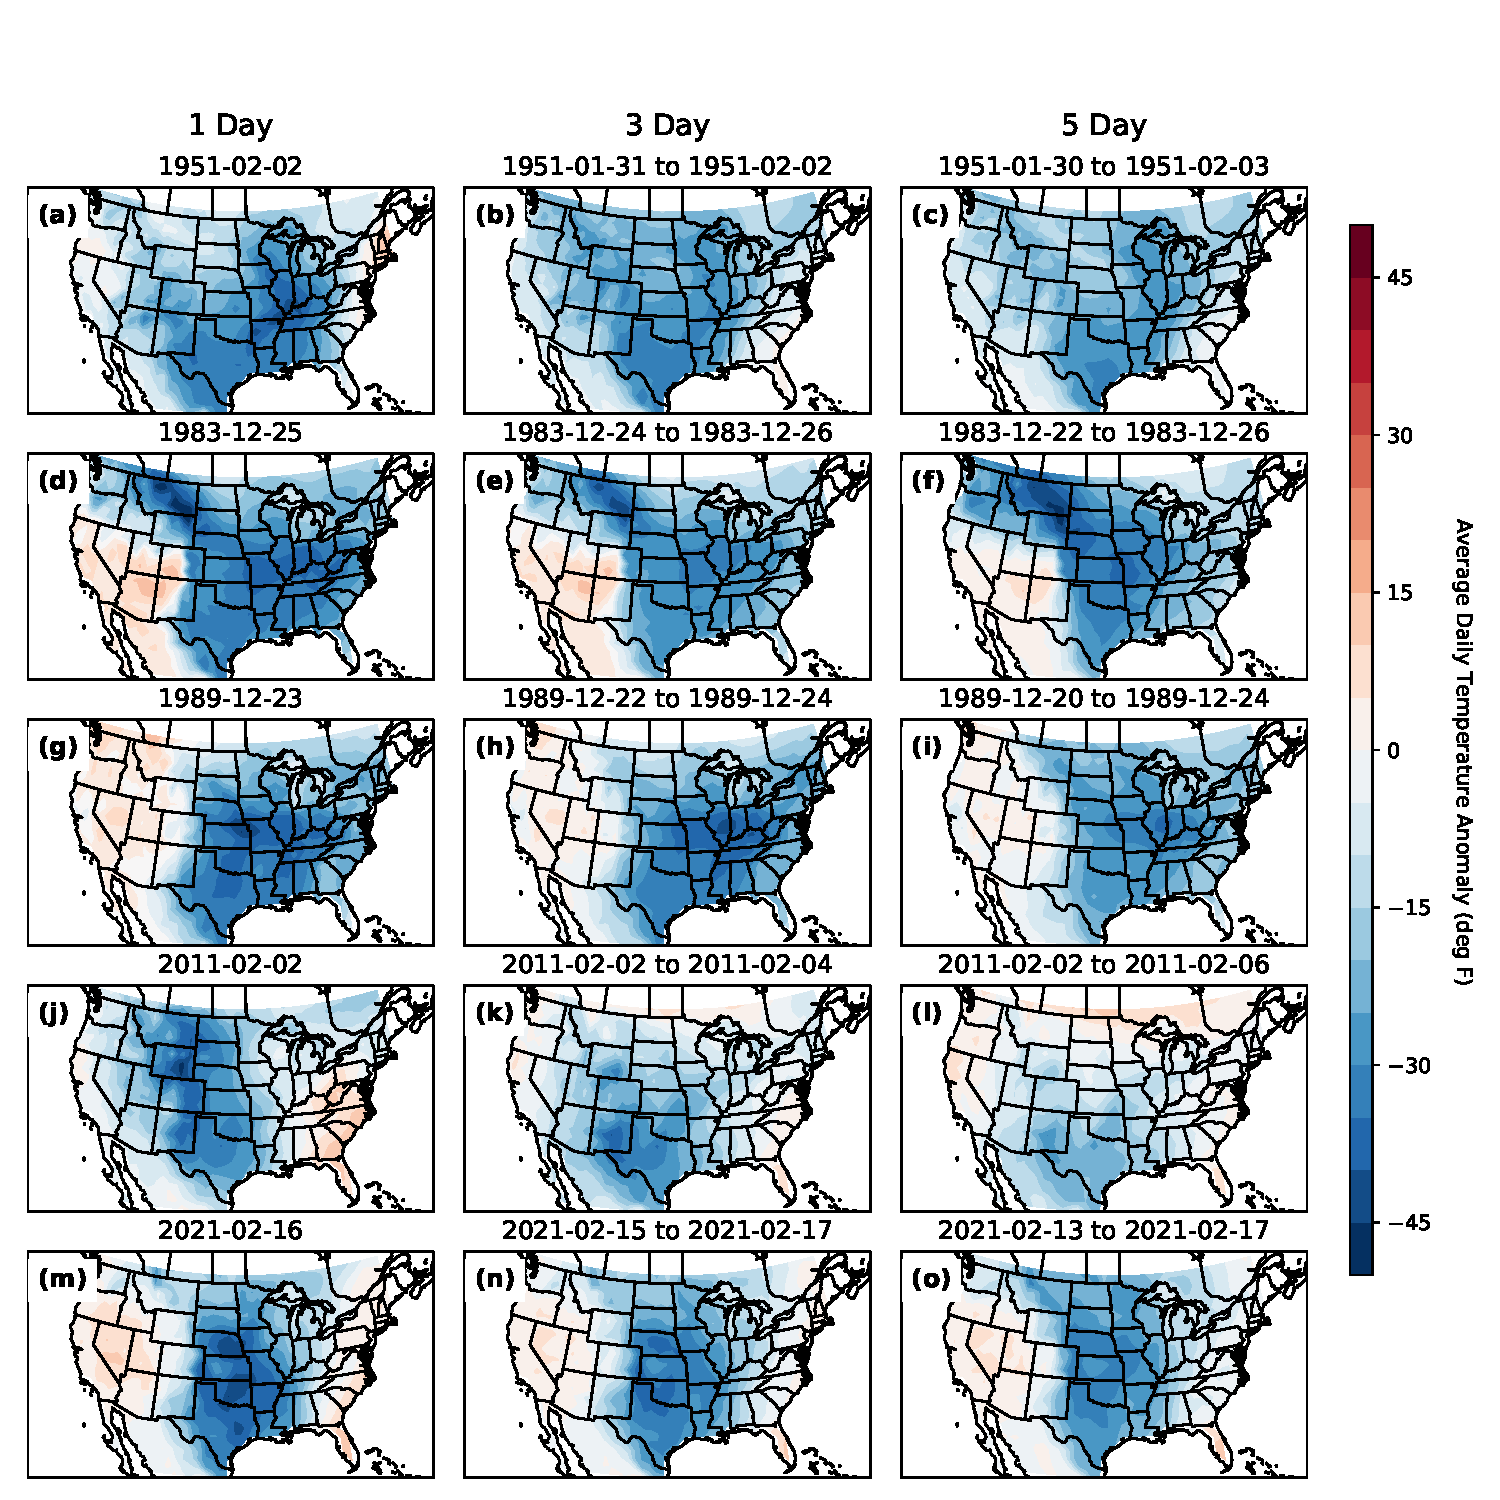
\includegraphics[width=\textwidth]{historic_events_era5.pdf}
  \caption{
    Severe cold snaps that affect Texas and extend into the central United States have several precedents in the historical record.
    Plot shows anomalies of daily mean temperatures \DIFaddbeginFL \DIFaddFL{from the ERA-5 reanalysis \mbox{%DIFAUXCMD
        \cite{hersbach_era5:2020} }\hspace{0pt}%DIFAUXCMD
    }\DIFaddendFL for historic major cold events affecting Texas, defined as the departure from the seasonal (December-February) mean \DIFdelbeginFL \DIFdelFL{to facilitate comparison }\DIFdelendFL of \DIFdelbeginFL \DIFdelFL{events in different calendar months.
      Temperatures over }\DIFdelendFL the \DIFdelbeginFL \DIFdelFL{Continental United States are plotted to show }\DIFdelendFL \DIFaddbeginFL \DIFaddFL{observational record.
      Anomalies facilitate identification of }\DIFaddendFL large-scale \DIFaddbeginFL \DIFaddFL{weather }\DIFaddendFL patterns \DIFdelbeginFL \DIFdelFL{, but events are selected based only }\DIFdelendFL \DIFaddbeginFL \DIFaddFL{superimposed }\DIFaddendFL on \DIFdelbeginFL \DIFdelFL{Texas temperatures}\DIFdelendFL \DIFaddbeginFL \DIFaddFL{long-term climatological averages}\DIFaddendFL .
    Hourly temperatures are averaged to 1-day (a,d,g,j,m), 3-day (b,e,h,k,n), and 5-day (c,f,i,l,o) average temperature anomalies.
  }\label{fig:historic_era5}
\end{figure}

\section{Data and Methods}

We use three distinct datasets to analyze temperature minima in \DIFdelbegin \DIFdel{Texas }\DIFdelend \DIFaddbegin \DIFadd{the region covered by the Texas Interconnection }\DIFaddend through the lens of distributed (each grid cell analyzed separately) and aggregated (weighted averages taken across space) extreme values analysis.

\subsection{Datasets}

We use three temperature datasets to ensure robust findings:
\begin{enumerate}
  \item Hourly \SI{2}{\meter} air temperature reanalysis on a \SI{0.25}{\degree} grid from the ERA-5 reanalysis project produced by the European Centre for Medium Range Weather Forecasting \cite{hersbach_era5:2020} and available  from the Copernicus Data Store (\url{https://cds.climate.copernicus.eu}) from 1950 to the present.
        The period from 1950 to 1979 is released as a preliminary back extension.
        All plots shown in the main text use the ERA-5 data, but supplemental figures use other data sets.
  \item Daily mean, minimum and maximum temperatures, gridded to \SI{1}{\degree}, produced by Berkeley Earth (\url{http://berkeleyearth.org/data/}).
        This gridded product is based on statistical analysis of station data and is available from 1880 to 2019.
        This dataset is considered an experimental product, so we use it only for comparative purposes.
  \item To complement blended gridded data products, we use station temperature data from the Global Historical Climatology Network (GHCN) dataset compiled by the National Ocean and Atmospheric Administration \cite{Menne:2012hk} and available at \url{https://www1.ncdc.noaa.gov/pub/data/ghcn/daily/}.
        This dataset provides daily mean, maximum, and minimum temperature observations.
        These measurements represent point measurements, which can differ in important ways from gridded products describing spatial averages due to the spatial heterogeneity of temperature fields.
        We retain stations within the state of Texas if they provide at least 60 years of data and if they contain observations for the set of historical cold extremes shown in \cref{fig:historic_era5}.
\end{enumerate}
We also use population density data from the GPWv4 dataset \cite{ciesin_gpwv4:2016}, a list of power generation facilities from the US Energy Information Administration \cite{useia_generators:2021}, and a map of the Texas \DIFdelbegin \DIFdel{Interconnect }\DIFdelend \DIFaddbegin \DIFadd{Interconnection }\DIFaddend \cite{useia_regions:2021}.


\subsection{Inferred \DIFdelbegin \DIFdel{Demand for Heating}\DIFdelend \DIFaddbegin \DIFadd{heating demand per capita}\DIFaddend }\label{sec:inferred-demand}

Most space heating in Texas is either electric or gas \cite{waite_heating:2020} and the majority of power generation in the Texas \DIFdelbegin \DIFdel{Interconnect }\DIFdelend \DIFaddbegin \DIFadd{Interconnection }\DIFaddend depends on natural gas \cite{everhart_iea:2021}.
Stress on natural gas production and delivery was therefore just as important as the more visible stress on the electric system \DIFaddbegin \DIFadd{\mbox{%DIFAUXCMD
    \cite{ercotpublic_outagesv2:2021}}\hspace{0pt}%DIFAUXCMD
}\DIFaddend .

The hourly or daily thermal energy requirement for space heating is primarily driven by how much lower the ambient temperature is than an indoor comfort temperature of \DIFdelbegin \DIFdel{\mbox{%DIFAUXCMD
    \SI{68}{\degree F}}\hspace{0pt}%DIFAUXCMD
}\DIFdelend \DIFaddbegin \DIFadd{\mbox{%DIFAUXCMD
    \SI{65}{\degree F}}\hspace{0pt}%DIFAUXCMD
}\DIFaddend .
This relationship is often expressed in terms of heating degree days or hours.
We therefore consider the \DIFdelbegin \DIFdel{temperature excursion from \mbox{%DIFAUXCMD
    \SI{68}{\degree F} }\hspace{0pt}%DIFAUXCMD
}\DIFdelend \DIFaddbegin \DIFadd{difference between observed temperatures and a standard indoor temperature of \mbox{%DIFAUXCMD
    \SI{65}{\degree F} }\hspace{0pt}%DIFAUXCMD
}\DIFaddend as a proxy for thermal heating demand.
We compute this value each hour for the ERA5 data, defining heating demand at each grid cell as \DIFdelbegin \DIFdel{$\text{HD}_t = \max (68 - T_t, 0)$}\DIFdelend \DIFaddbegin \DIFadd{$\text{HD}_t = \max (65 - T_t, 0)$}\DIFaddend , where $T_t$ is the temperature at hour $t$ in \si{\degree F}.
The Berkeley Earth and GHCN datasets provide daily minimum and maximum temperatures, so we define heating demand at each grid cell or station as \DIFdelbegin \DIFdel{$\text{HD}_d = \max (68 -\frac{T_{\text{min},d} + T_{\text{max},d}}{2}, 0)$}\DIFdelend \DIFaddbegin \DIFadd{$\text{HD}_d = \max (65 -\frac{T_{\text{min},d} + T_{\text{max},d}}{2}, 0)$}\DIFaddend , where $T_{\text{min},d}$ is the minimum temperature recorded on day $d$ and $T_{\text{max},d}$ is the maximum temperature recorded on day $d$, both in \si{\degree F}.

To assess how spatially correlated cold spells might affect the Texas electric grid, we average heating demand in space over the Texas \DIFdelbegin \DIFdel{Interconnect }\DIFdelend \DIFaddbegin \DIFadd{Interconnection }\DIFaddend domain \cite{useia_regions:2021}, weighting each grid cell by 2020 population density \cite{ciesin_gpwv4:2016}.
We refer to this spatially aggregated time series, which has the straightforward interpretation as the average heating demand experienced by Texas residents, as ``Inferred \DIFdelbegin \DIFdel{Demand for Heating }\DIFdelend \DIFaddbegin \DIFadd{Heating Demand per Capita}\DIFaddend .''

\subsection{Return Period}

\DIFaddbegin \DIFadd{Return periods define the probability with which a particular event can be expected to occur.
  Thus, a $T$-year event has a $\frac{1}{T}$ probability of occurring in a given year.
}\DIFaddend For each event duration considered, \DIFdelbegin \DIFdel{return periods are obtained }\DIFdelend \DIFaddbegin \DIFadd{we calculated return periods }\DIFaddend by fitting a stationary generalized extreme value (GEV) distribution to the time series of annual \DIFdelbegin \DIFdel{minimum December-February (DJF) temperatures, or to the time series of annual }\DIFdelend maxima of inferred \DIFdelbegin \DIFdel{demand for heating (}\DIFdelend \DIFaddbegin \DIFadd{heating demand per capita (see }\DIFaddend \cref{sec:inferred-demand}).
Events that occur in December are coded to the following year \DIFaddbegin \DIFadd{so that a single winter season is grouped together}\DIFaddend .
The 2021 winter season was excluded from return period estimates, allowing us to interpret return periods for the February 2021 event as \emph{a priori} estimates.

\subsection{Cold Duration}

The effect of cold temperatures on energy demand and critical infrastructure depends on how long the cold persists.
Short duration cold snaps can kill plants, freeze exposed pipes, freeze wind turbines, and contribute to dangerous roadway conditions.
Longer duration cold spells contribute to demand for heating and energy and cause pipes to burst even if they have some insulation.
We calculate demand for heating by taking temporal averages over a range of durations from 1 hour to 4 days.

\subsection{Code and Data}

We are committed to open science.
Our open source code is freely available in a live repository at \url{https://github.com/jdossgollin/2021-TXtreme} and in an archived repository at \url{https://dx.doi.org/10.5281/zenodo.4568923}.
Reproducibility is facilitated through the Snakemake library \cite{koster_snakemake:2012}.

\section{How extreme was inferred heating demand \DIFaddbegin \DIFadd{per capita }\DIFaddend over the Texas \DIFdelbegin \DIFdel{Interconnect}\DIFdelend \DIFaddbegin \DIFadd{Interconnection}\DIFaddend ?}

The total shock to Texas heating demand is partially determined by the extent to which cold snaps impact multiple population centers simultaneously.
As such, understanding whether there was precedent for a cold snap simultaneously affecting several regions of Texas's grid that today have high population density is critical.
We therefore use our measure of inferred \DIFdelbegin \DIFdel{demand for heating }\DIFdelend \DIFaddbegin \DIFadd{heating demand per capita }\DIFaddend (see \cref{sec:inferred-demand}) to represent the aggregate heating demand induced by cold temperatures.
Aggregating historic temperature fields in space using the 2020 population, we answer the question ``what would the aggregate demand for heating have been had historic cold snaps occurred today?''

\Cref{fig:idf_weighted} shows that the intensity, duration, and recurrence intervals of the February 2021 storm are severe but not unprecedented in the historical record.
For example, at the 6 hour duration the December 1989 storm was substantially more intense and other storms including February 1951 were nearly as intense.
At the two day duration, the 2021 and 1989 events were approximately equally intense and other storms including December 1983 were nearly as intense.
The 2011 storm, which caused rolling blackouts and motivated research into the energy system's vulnerability to cold \cite{ferc_outages:2011}, was quite modest by comparison.
The right panel shows statistical return periods for these extreme events\DIFdelbegin \DIFdel{, though these estimates are sensitive to small changes in inferred demand for heating}\DIFdelend .

\begin{figure}
  \centering
  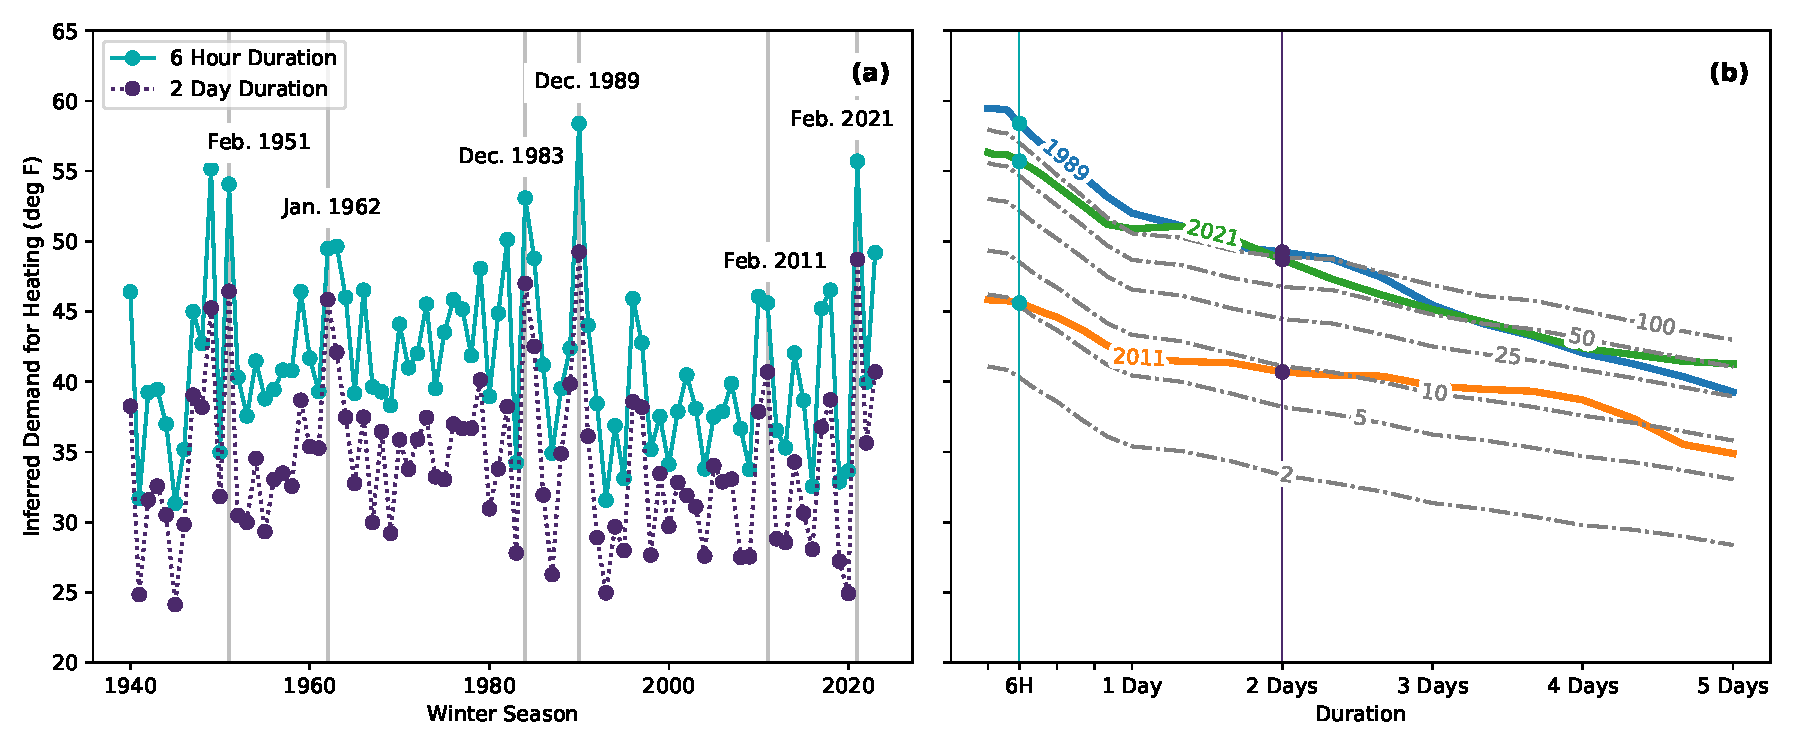
\includegraphics[width=\textwidth]{ERCOT_HDD_IDF_MLE_popweighted.pdf}
  \caption{
    The inferred \DIFdelbeginFL \DIFdelFL{demand for }\DIFdelendFL heating \DIFaddbeginFL \DIFaddFL{demand per capita }\DIFaddendFL induced by the February 2021 cold snap is not unprecedented.
    For the worst 6 hours, the 1989 event was more severe than the 2021 event, while they are comparable for \DIFdelbeginFL \DIFdelFL{the }\DIFdelendFL longer durations.
    (a): time series of annual maximum inferred \DIFdelbeginFL \DIFdelFL{demand for }\DIFdelendFL heating \DIFaddbeginFL \DIFaddFL{demand per capita }\DIFaddendFL (\cref{sec:inferred-demand}) at 6 hour and 2 day durations.
    December extremes, including the December 1989 storm, are coded to the following year so that one maximum per December-February winter season is taken.
    (b): the intensity-duration-frequency intervals estimated using 1950-2020 data (i.e., not using the 2021 event), overlaid by the annual maxima from the 1989, 2011, and 2021 events.
    Gray dashed lines indicate 2, 5, 10, 25, 50, and 100 year return levels.
  }\label{fig:idf_weighted}
\end{figure}

\section{Spatially distributed temperature extremes}

It is difficult to establish a spatially aggregated proxy for supply-side risk given complex interlinkages between natural gas, electric, and other systems which create the possibility for cascading failures as observed in February 2021.
Water treatment and distribution systems, as well as other essential services, also rely on electricity, further increasing vulnerabilities.
Instead of aggregating this risk in space, we estimate the exceedance probability of the February 2021 temperatures at each grid cell separately to shed light on the severity of cold experienced by installations across the region.

\Cref{fig:local_era5} shows local return periods for the February 2021 cold snap at 6 hour, 1 day, 2 day, and 4 day durations.
Other than a band from south-central to south-east Texas, nearly all regions of the Texas \DIFdelbegin \DIFdel{Interconnect }\DIFdelend \DIFaddbegin \DIFadd{Interconnection }\DIFaddend (gray outline in \cref{fig:local_era5}a,d) experienced cold with a return period below 50 years.
Results are similar using station data (\cref{fig:local_ghcnd}).
Importantly for the energy system, the band experiencing cold with return period greater than 50 years includes a substantial fraction of Texas’s population (\cref{fig:local_era5}a) and natural gas generation (\cref{fig:local_era5}d).
Outside the Texas \DIFdelbegin \DIFdel{Interconnect region, much of the }\DIFdelend \DIFaddbegin \DIFadd{Interconnection region, the Midcontinent Independent System Operator and Southwest Power Pool instructed utilities to shed firm load, but of the approximately 4.89 million customers without power in Texas, Louisiana, and Oklahoma, an estimated 4.5 million were in }\DIFaddend Texas \DIFdelbegin \DIFdel{Panhandle and central Oklahomaexperienced intense cold with a return period greater than 100 years at multiple durations.
  Although Oklahoma recorded some water main breaks \mbox{%DIFAUXCMD
    \cite{crum_water:2021} }\hspace{0pt}%DIFAUXCMD
  and rolling blackouts for several hours \mbox{%DIFAUXCMD
    \cite{money_oklahoma:2021}}\hspace{0pt}%DIFAUXCMD
  , infrastructure impacts were less severe than in Texas despite recording more extreme (relative both to its own historical record and in absolute terms) temperatures}\DIFdelend \DIFaddbegin \DIFadd{\mbox{%DIFAUXCMD
    \cite{ceser_winterupdate:2021}}\hspace{0pt}%DIFAUXCMD
}\DIFaddend .

\begin{figure}
  \centering
  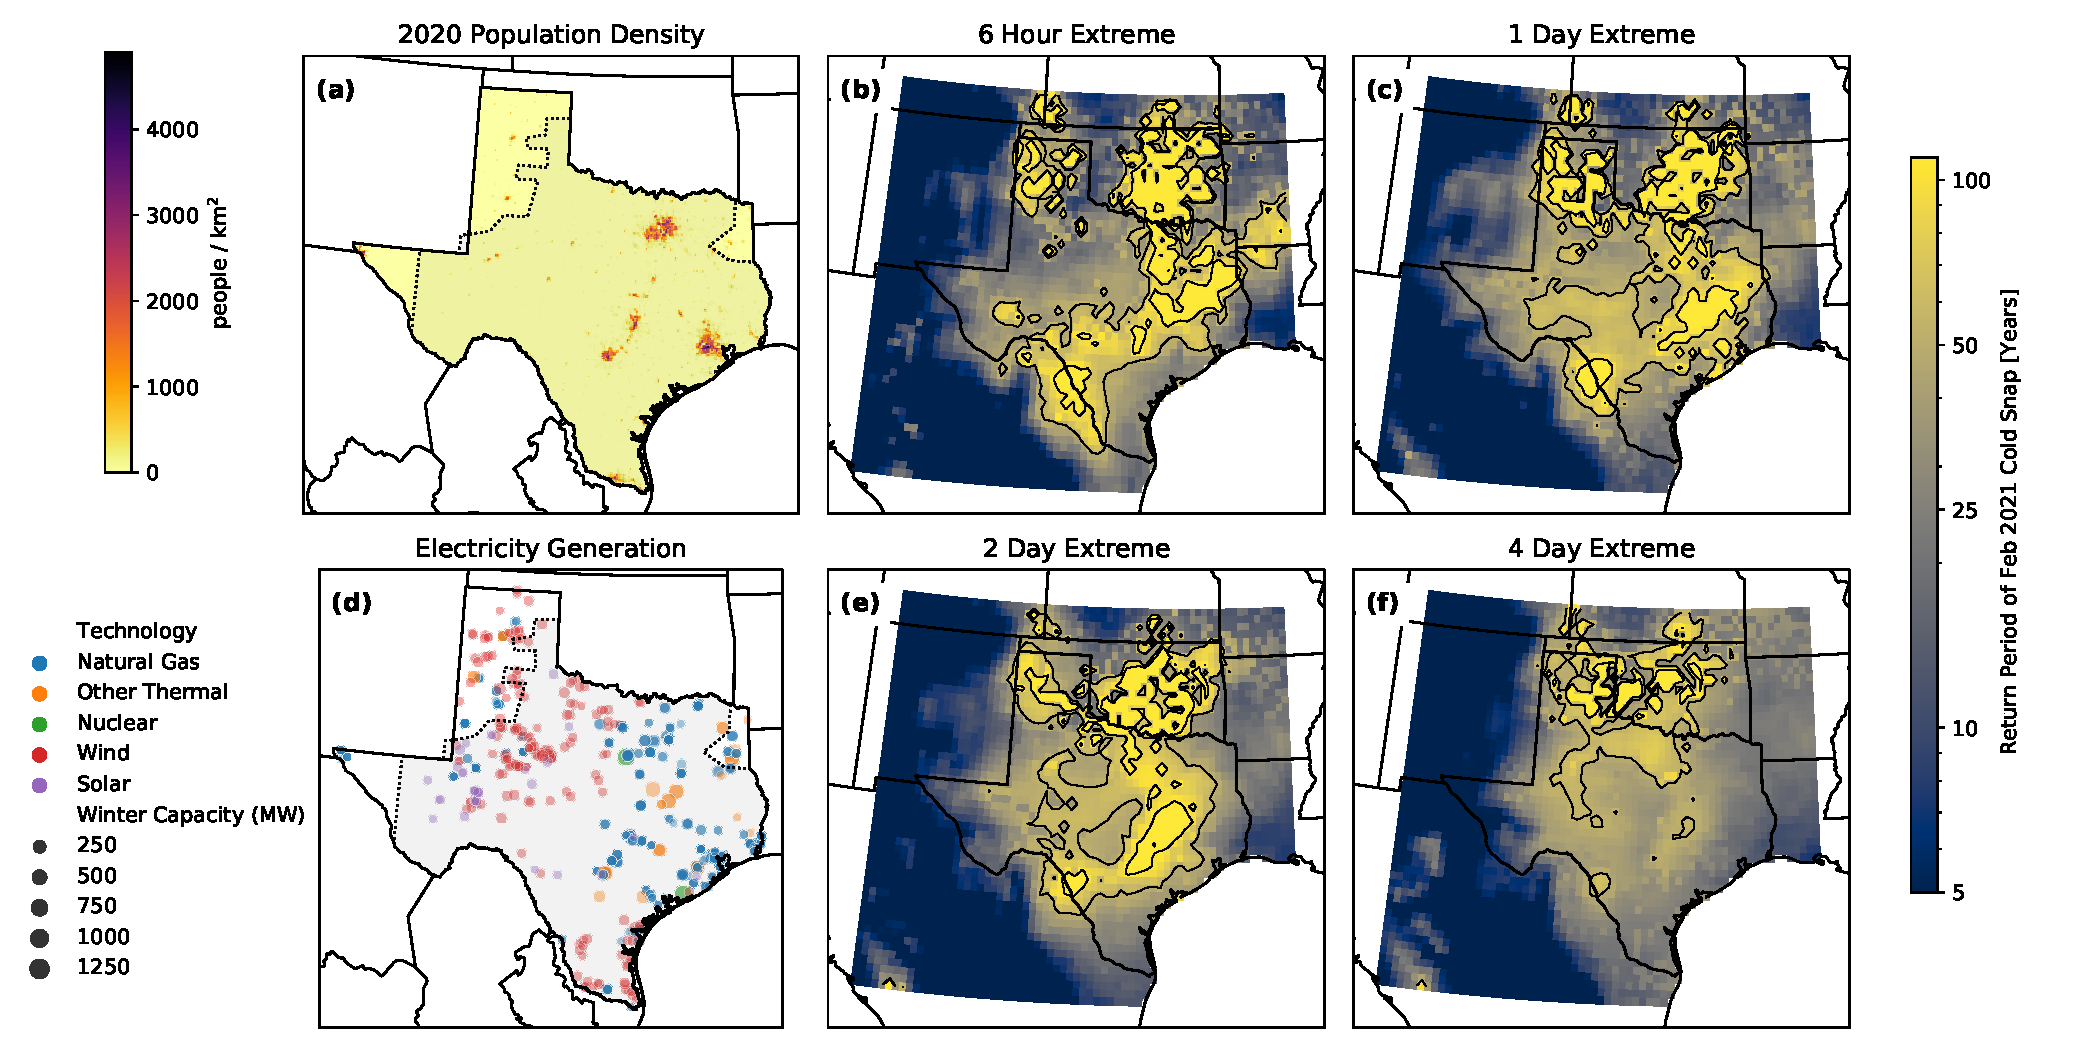
\includegraphics[width=\textwidth]{local_rt_era5.pdf}
  \caption{
    Return periods for the February 2021 event, calculated using stationary estimates of annual extremes over the period 1950-2020.
    Return periods are calculated separately for each cell.
    (a): estimates of 2020 population density \cite{ciesin_gpwv4:2016}.
    (d): energy generation facilities in Texas \cite{useia_generators:2021}.
    (b,c,e,f): local return periods for 6 hour, 1 day, 2 day, and 4 day durations, respectively.
    Contours enclose regions that recorded 50 and 100 year return levels.
    The gray region in panels (a) and (d) shows boundaries of the Texas \DIFdelbeginFL \DIFdelFL{Interconnect }\DIFdelendFL \DIFaddbeginFL \DIFaddFL{Interconnection }\DIFaddendFL \cite{useia_regions:2021}.
  }\label{fig:local_era5}
\end{figure}

\section{Discussion}

Our spatially aggregated metric of inferred \DIFdelbegin \DIFdel{demand for heating }\DIFdelend \DIFaddbegin \DIFadd{heating demand per capita }\DIFaddend shows that the February 2021 event was intense but not unforeseeable (\cref{fig:idf_weighted}).
Although specific locations experienced very intense ($>100$ year return period) temperatures, we find that for most locations in Texas the temperatures recorded during the February 2021 cold snap had precedent in the historical record\DIFdelbegin \DIFdel{and could have been anticipated given available data}\DIFdelend .

A proximate cause of load shedding in the Texas \DIFdelbegin \DIFdel{Interconnect }\DIFdelend \DIFaddbegin \DIFadd{Interconnection }\DIFaddend during February 2021 was the vulnerability of the electricity generation system to the severe cold temperatures \cite{everhart_iea:2021}.
\DIFdelbegin \DIFdel{\mbox{%DIFAUXCMD
    \Cref{fig:local_era5,fig:local_ghcnd} }\hspace{0pt}%DIFAUXCMD
  show that this happened }\DIFdelend \DIFaddbegin \DIFadd{As shown in \mbox{%DIFAUXCMD
    \cref{fig:egova}}\hspace{0pt}%DIFAUXCMD
  , generator outages occurred across the state, }\DIFaddend even though most parts of the state had previously experienced similarly intense cold, notably in \DIFdelbegin \DIFdel{1989.
}\DIFdelend \DIFaddbegin \DIFadd{1989 (\mbox{%DIFAUXCMD
    \cref{fig:local_era5,fig:local_ghcnd}}\hspace{0pt}%DIFAUXCMD
  ).
  Yet despite temperatures that were, in aggregate, more intense, the electricity system experienced fewer than three hours of rolling blackouts from December 21-23, 1989 \mbox{%DIFAUXCMD
    \cite{nerc_operation:1989,osborne_twofreezes:2021}}\hspace{0pt}%DIFAUXCMD
  .
  Following the 1983, 1989, and 2011 cold snaps, the North American Electric Reliability Corporation (NERC) warned that ``constraints on natural gas fuel supplies to generating plants'' and ``generating unit trips, derates, or failure to start due to weather related causes'' were common themes across severe and moderate cold extremes \mbox{%DIFAUXCMD
    \cite{nerc_previous:2013}}\hspace{0pt}%DIFAUXCMD
  , foreshadowing many of the causes of February 2021 energy system failures identified by ERCOT \mbox{%DIFAUXCMD
    \cite{ercotpublic_outagesv2:2021,magness_review:2021}}\hspace{0pt}%DIFAUXCMD
  .
}\DIFaddend While our analysis neglects other meteorological factors, like freezing rain, that may have impeded operations at specific facilities, \DIFdelbegin \DIFdel{our analysis suggests }\DIFdelend \DIFaddbegin \DIFadd{we find }\DIFaddend that the February 2021 failures of energy and electricity systems in the Texas \DIFdelbegin \DIFdel{Interconnect }\DIFdelend \DIFaddbegin \DIFadd{Interconnection }\DIFaddend took place during temperatures \DIFdelbegin \DIFdel{comparable to those previously recorded.
  Similarly, water mains broke in places like Houston where temperatures did not exceed 100-year return levels, underscoring characteristic vulnerability of critical infrastructure systems \mbox{%DIFAUXCMD
    \cite{chester_reliable:2020}}\hspace{0pt}%DIFAUXCMD
}\DIFdelend \DIFaddbegin \DIFadd{with precedent in the historical record}\DIFaddend .

Another cause of load shedding was the high demand for electricity that low temperatures induced.
Currently \DIFdelbegin \DIFdel{over }\DIFdelend \DIFaddbegin \DIFadd{at least }\DIFaddend 50\% of Texas households use electricity for space heating over the majority of census tracts of the state \cite{waite_heating:2020} and further electrification is a central element of many plans to decarbonize our energy sector \cite{williams_decarbonization:2012,davis:2018,white_txresidential:2019}.
While summer peak loads have been a central planning concern on the Texas grid in the past, it is likely that winter peak loads will become a greater concern in the coming decades.
In fact, the \DIFdelbegin \DIFdel{peak demand }\DIFdelend \DIFaddbegin \DIFadd{estimated \mbox{%DIFAUXCMD
    \SI{76819}{\mega\watt} }\hspace{0pt}%DIFAUXCMD
  of peak demand without load shedding }\DIFaddend during this event \DIFdelbegin \DIFdel{was estimated at around \mbox{%DIFAUXCMD
    \SI{74.5}{\giga\watt}}\hspace{0pt}%DIFAUXCMD
  , just shy of the all time peak for any season of \mbox{%DIFAUXCMD
    \SI{74.8}{\giga\watt} }\hspace{0pt}%DIFAUXCMD
  in August }\DIFdelend \DIFaddbegin \DIFadd{\mbox{%DIFAUXCMD
    \cite{magness_review:2021} }\hspace{0pt}%DIFAUXCMD
  exceeded not only the previous winter demand record of \mbox{%DIFAUXCMD
    \SI{65900}{\mega\watt} }\hspace{0pt}%DIFAUXCMD
  recorded on January 17, 2018 but also the all-season record actual demand of \mbox{%DIFAUXCMD
    \SI{74800}{\mega\watt} }\hspace{0pt}%DIFAUXCMD
  recorded on August 19, }\DIFaddend 2019 \cite{everhart_iea:2021}.
As electrification of heating \DIFdelbegin \DIFdel{increases}\DIFdelend \DIFaddbegin \DIFadd{continues}\DIFaddend , severe cold snaps may \DIFaddbegin \DIFadd{consistently }\DIFaddend represent the peak demand on the Texas Interconnect.

Our primary findings hold for an alternative gridded dataset and station data (see supplemental material).
However, calculated return periods are sensitive to the method of estimation (\cref{fig:idf_lmoments_unweighted,fig:idf_lmoments_weighted}).
Future analysis could address parametric uncertainty, model structure uncertainty \cite{wong_floodrisk:2018}, non-stationarity \cite{Milly:2008dg}, or regime-like modes of climate variability \cite{DossGollin:2019}.
More fundamentally, an assessment of exposure to cold extremes over the next decades should consider the deeply uncertain distribution of future climate change, and the induced effect on cold extremes in Texas.
Although a broad scientific consensus suggests the frequency of cold extremes should decrease under warming in most places \cite{ipcc_ar5:2014}, possible links between North-South temperature gradients and mid-latitude temperature extremes remains an area of active research \DIFdelbegin \DIFdel{\mbox{%DIFAUXCMD
    \cite{Barnes:2013fp,Cohen:2014gx,Screen:2013ho}}\hspace{0pt}%DIFAUXCMD
}\DIFdelend \DIFaddbegin \DIFadd{\mbox{%DIFAUXCMD
    \cite{Barnes:2013fp,Cohen:2014gx,Screen:2013ho,romanowsky_stratosphere:2019}}\hspace{0pt}%DIFAUXCMD
}\DIFaddend .
Regardless, the effect of climate change on peak demand for heating is likely to be small compared to the effect of rapid population growth \DIFdelbegin \DIFdel{; for example, }\DIFdelend \DIFaddbegin \DIFadd{which }\DIFaddend the Texas Water Development Board\DIFdelbegin \DIFdel{anticipates at least }\DIFdelend \DIFaddbegin \DIFadd{, for example, anticipates to be }\DIFaddend 40\% \DIFdelbegin \DIFdel{growth }\DIFdelend from 2020 to 2050 \cite{texaswaterplan:2012}.

Our analysis quantifies the \DIFdelbegin \DIFdel{probability with which temperature extremes }\DIFdelend \DIFaddbegin \DIFadd{frequency with which the temperatures observed during February 2021 }\DIFaddend could have been \DIFdelbegin \DIFdel{anticipated }\DIFdelend \DIFaddbegin \DIFadd{expected to occur }\DIFaddend \emph{a priori}.
Other factors also govern infrastructure performance and failure, including precipitation, the demand for natural gas in adjacent regions, and complex connections within and between regional systems.
Similarly, decisions at multiple time scales, including disaster preparedness and risk communication, contribute to the human consequences of physical infrastructure failure.
Thus, the exact chain of events that led to the blackouts and water system disruptions during February 2021 should be sorted out only after thorough investigations by parties on the ground in Texas.

\section{Conclusions}

The February 2021 cold snap was the most intense in 30 years, but was not without precedent in the full historical record.
In addition to the record cold conditions of 1899 (\cref{fig:historic_bk}), we estimate that the weather of December 1989 would have resulted in \DIFdelbegin \DIFdel{slightly }\DIFdelend higher 6-hour and 2-day \DIFdelbegin \DIFdel{aggregate heating demands }\DIFdelend \DIFaddbegin \DIFadd{values of inferred heating demand per capita }\DIFaddend over the Texas \DIFdelbegin \DIFdel{Interconnect had it occurred in February 2021.
  Several other storms since 1950 would have produced nearly as much demand for heating }\DIFdelend \DIFaddbegin \DIFadd{Interconnection than the February 2021 event.
  Storms in February 1951, January 1962, and December 1983 would have resulted in at least 90\% as much inferred heating demand per capita}\DIFaddend .
Given upward trends in the electrification of heating, it is likely that future cold snaps will cause peak annual loads on the Texas \DIFdelbegin \DIFdel{Interconnect }\DIFdelend \DIFaddbegin \DIFadd{Interconnection }\DIFaddend to occur during the winter season.
Infrastructure expansion necessitated by a rapidly growing population offers Texas the opportunity to invest in a more resilient energy system.

\section*{Acknowledgements}

DJF was supported by a gift from Gates Ventures LLC to the Carnegie Institution for Science.
The authors thank
\DIFaddbegin \DIFadd{Daniel Cohan,
}\DIFaddend Sylvia Dee,
Elisabeth Gawthrop,
\DIFaddbegin \DIFadd{Pedram Hassanzadeh,
  Fred Heutte,
}\DIFaddend Adam Massmann,
\DIFaddbegin \DIFadd{Alison Silverstein,
}\DIFaddend and
Vivek Srikrishnan
for \DIFdelbegin \DIFdel{comments on a preliminary draft of this manuscript}\DIFdelend \DIFaddbegin \DIFadd{discussion of this work}\DIFaddend .
The authors also thank the developers and maintainers of the open source packages we used, in particular the pydata and pangeo communities, and the many journalists and academics whose timely reporting and commentary has informed our thinking.

\section*{Bibliography}
\bibliographystyle{unsrt}
\bibliography{references}

\clearpage
\appendix
\section{Supplemental Results}
\renewcommand{\thefigure}{S\arabic{figure}}
\setcounter{figure}{0}

\subsection{Historic Extreme Temperatures}

To complement \cref{fig:historic_era5}, we plot extreme cold temperatures using alternate data.
First, \cref{fig:historic_bk} shows historic events over the Continental United States.
The set of events is slightly different than that of \cref{fig:historic_era5}: the data set does not include the 2021 event, but does include the 1899 ``Great Blizzard.''
The 1899 event shows more intense and persistent cold than the other events in the dataset.
Next, \cref{fig:historic_tx} shows the same data as \cref{fig:historic_era5} but zooms in on Texas.
The 1989 (g-i) and 2021 (m-o) appear to be the most severe events in this data set, and the 1-day cold extremes in the 1989 event are more intense than in the February 2021 event, consistent with results in the main text.

\begin{figure}
  \centering
  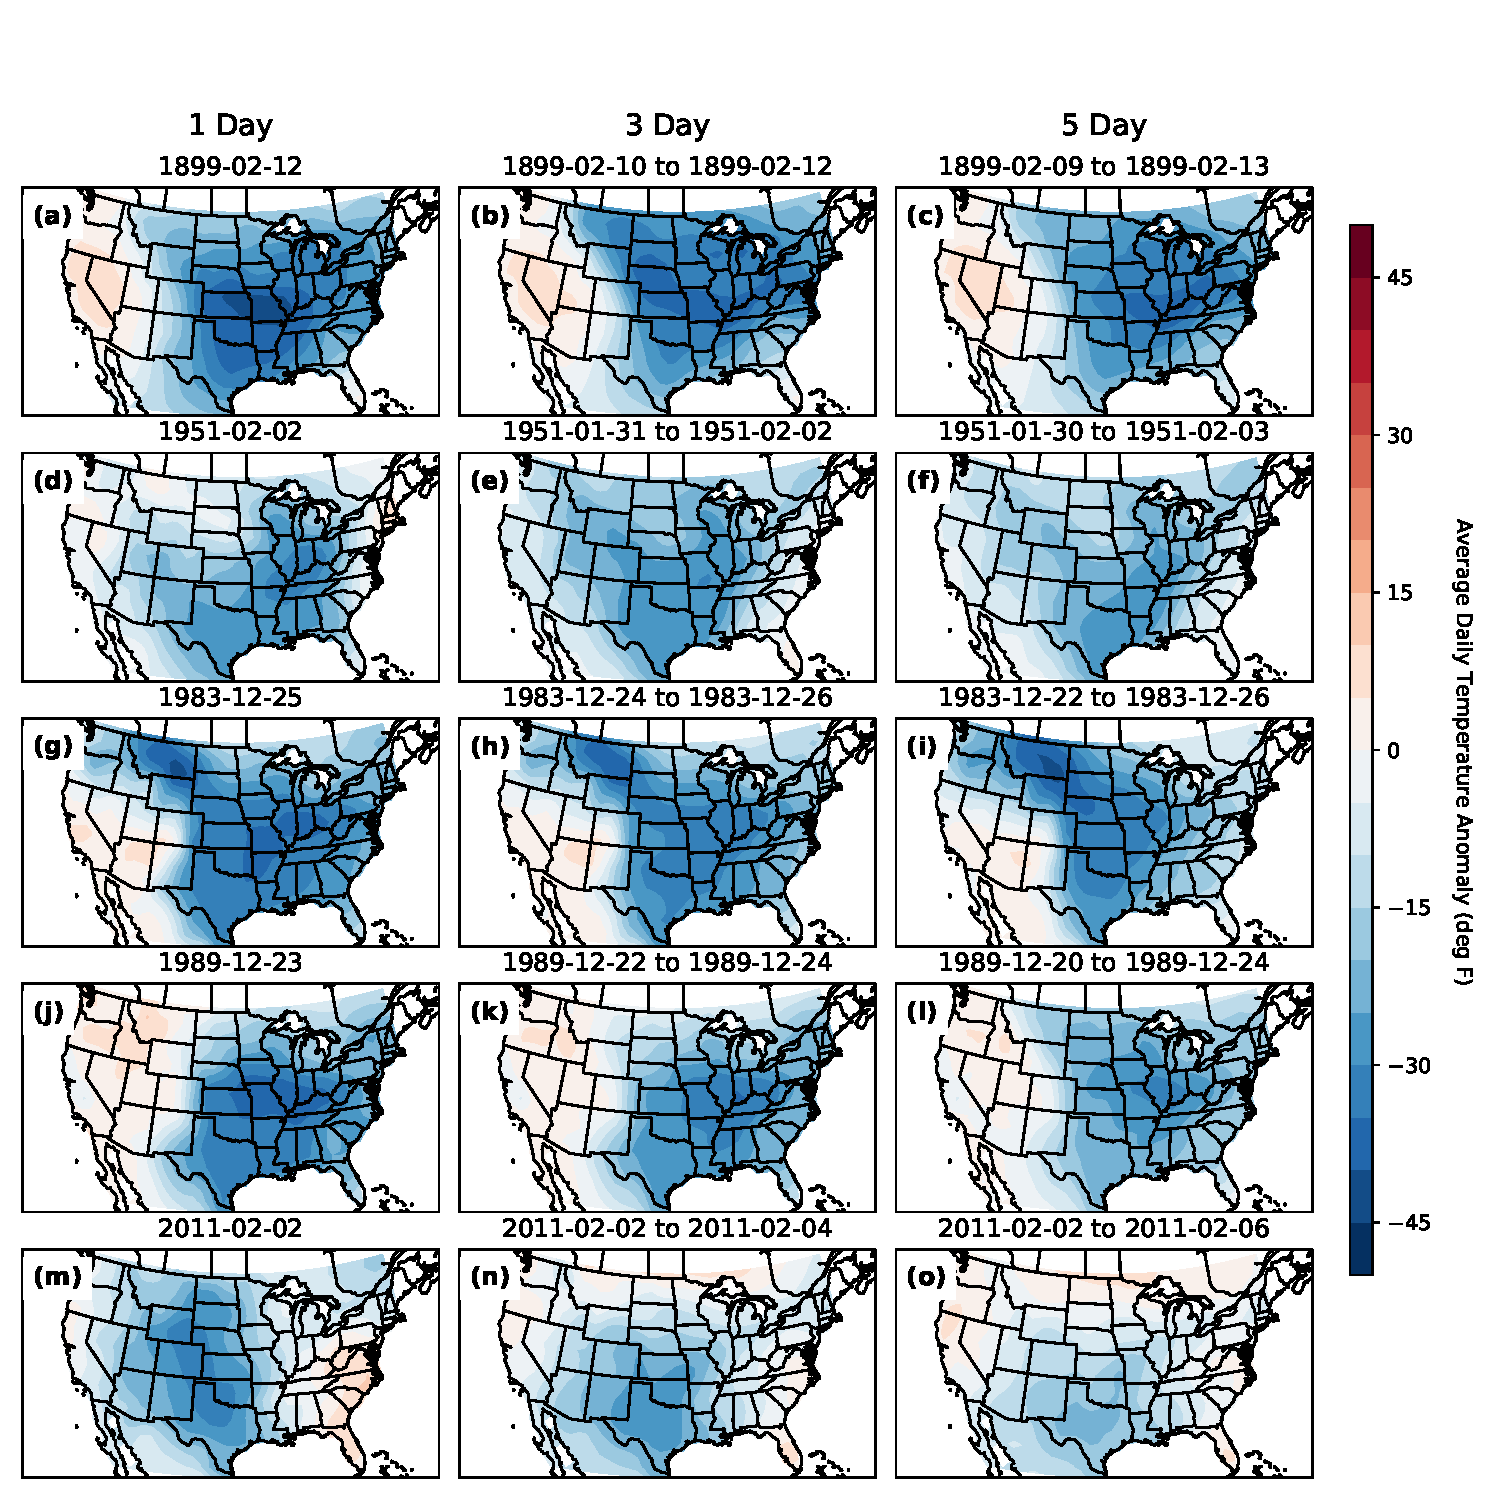
\includegraphics[width=\textwidth]{historic_events_bk.pdf}
  \caption{
    As \cref{fig:historic_bk} but the Berkely Earth temperature data is used.
    The dataset does not contain the 2021 event, but the ``Great Blizzard'' of February 1899 is included.
    Spatial patterns of cold from this dataset are qualitatively similar to Figure 1.
    The 1899 event emphasizes that the modern historical record does not yield a full sample from the full distribution of possible hazards.
  }\label{fig:historic_bk}
\end{figure}

\begin{figure}
  \centering
  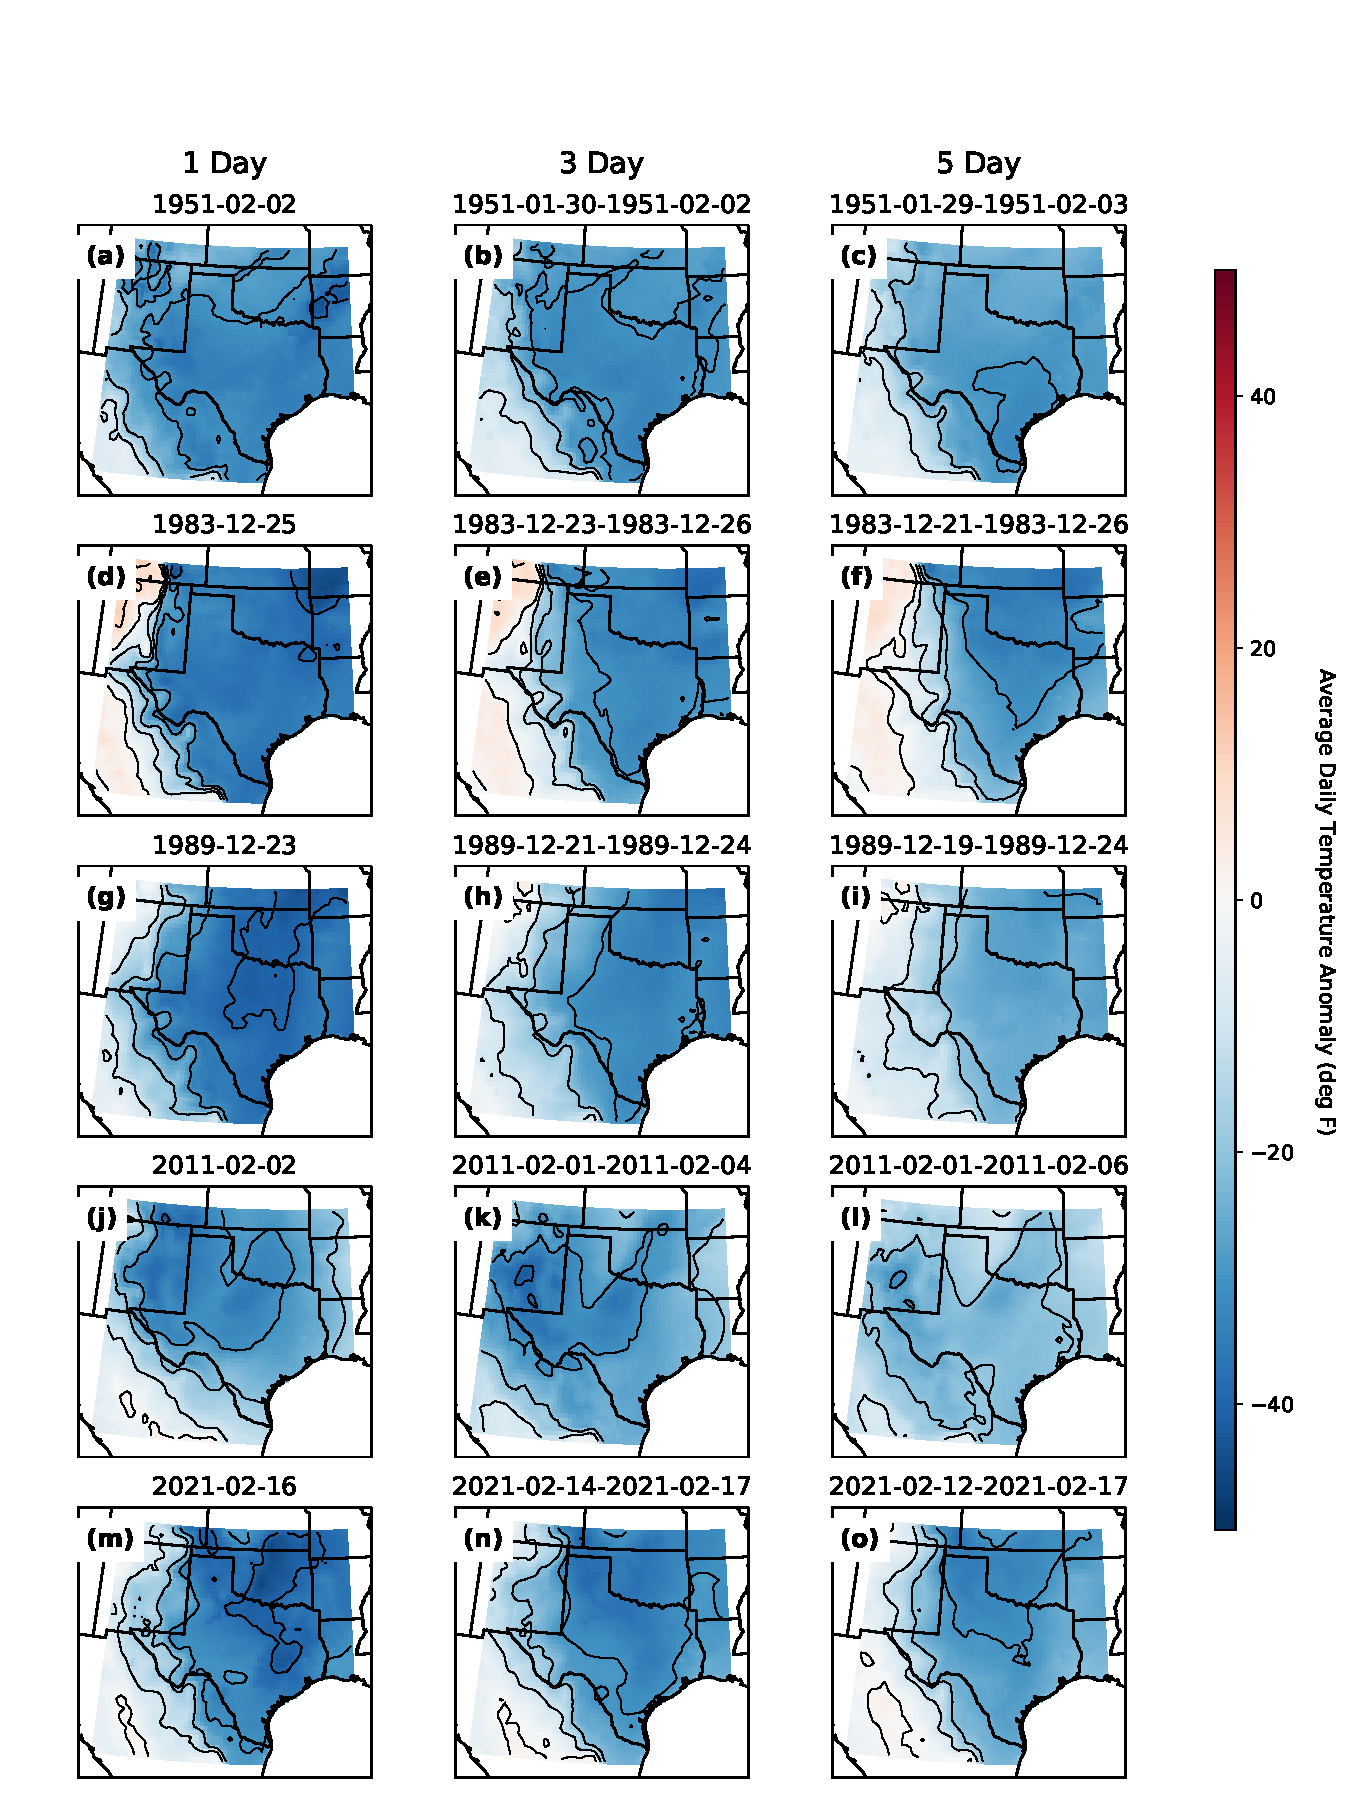
\includegraphics[width=\textwidth]{historic_events_era5_TX.pdf}
  \caption{
    As \cref{fig:historic_bk} but only Texas is shown.
  }\label{fig:historic_tx}
\end{figure}

\subsection{Spatially distributed temperature extremes}

To complement \cref{fig:local_era5}, we compute local return periods using station data from the GHCN \cite{Menne:2012hk}.
\Cref{fig:local_ghcnd} shows the return periods of the February 2021 cold snap for 1, 2, 3, and 4 day durations.
Only stations with at least 60 years of data are considered, and since the locations of these stations are not chosen at random, this does not constitute a representative sample of all points across Texas.
However, the spatial pattern matches that of \cref{fig:local_era5}, with a band of severe cold stretching from south-central to eastern Texas and in the Texas Panhandle.

\subsection{Inferred \DIFdelbegin \DIFdel{demand for }\DIFdelend heating \DIFaddbegin \DIFadd{demand per capita}\DIFaddend }

To complement our analysis of inferred \DIFdelbegin \DIFdel{demand for heating }\DIFdelend \DIFaddbegin \DIFadd{heating demand per capita}\DIFaddend , we consider how results change as a function of two modeling decisions.
First, we consider what happens if the spatial field demand for heating is aggregated using grid cell area rather than population density.
Next, we compute return periods using an estimator based on the method of $L$-moments.
Although $L$-moment estimators for the generalized extreme value distribution are not unbiased, they are popular in the statistical hydrology literature for their stability \cite{hosking_gev:1985,martins_gev:2001,morrison_gev:2002}.

We draw two conclusions from these plots.
First, the 2021 event appears more severe if grid cells are weighted by population density (\cref{fig:idf_weighted,fig:idf_lmoments_weighted}) than if they are weighted only by area \cref{fig:idf_unweighted,fig:idf_lmoments_unweighted}).
This is consistent with our observation of a correspondence between the most extreme temperatures in February 2021 and population density (\cref{fig:local_era5}).
By contrast, the 2011 event appears more extreme when grid cells are weighted by area, which is consistent with \cref{fig:historic_tx,fig:historic_era5,fig:historic_bk} showing the coldest temperatures in relatively less populated West Texas.
Second, the $L$-moment estimators (\cref{fig:idf_lmoments_weighted,fig:idf_lmoments_unweighted}) assign a lower return period to the 1989 and 2021 events than the maximum likelihood estimators (\cref{fig:idf_unweighted,fig:idf_weighted}).

To provide some context for our inferred demand for heating metric, \cref{fig:hdd_ts} plots its time series during the peak of the February 2021 cold snap.
This reveals a rise from approximately \SI{10}{\degree F} to nearly \SI{60}{\degree F} during the peak of the February 2021 cold snap.

\begin{figure}
  \centering
  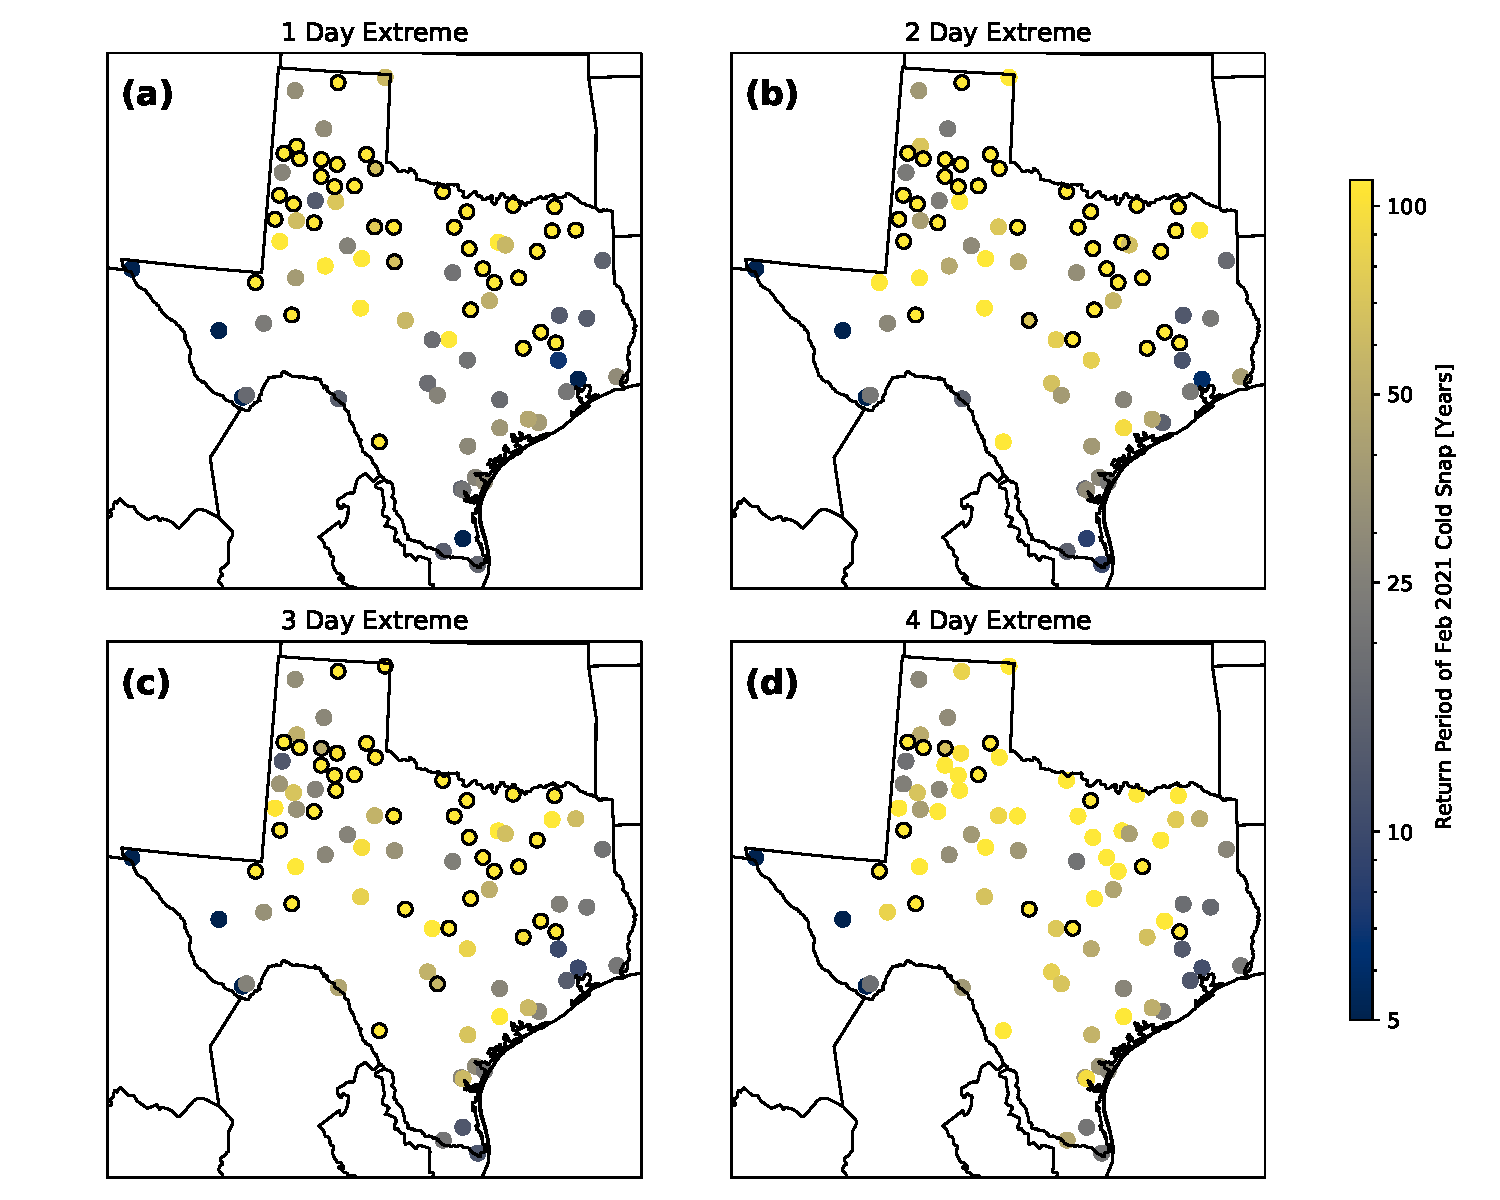
\includegraphics[width=\textwidth]{local_rt_ghcnd.pdf}
  \caption{
    As \cref{fig:local_era5} but return periods are calculated using station data from the GHCN data set \cite{Menne:2012hk}.
    Black circles indicate that a station exceeded its own record for a particular duration.
  }\label{fig:local_ghcnd}
\end{figure}

\begin{figure}
  \centering
  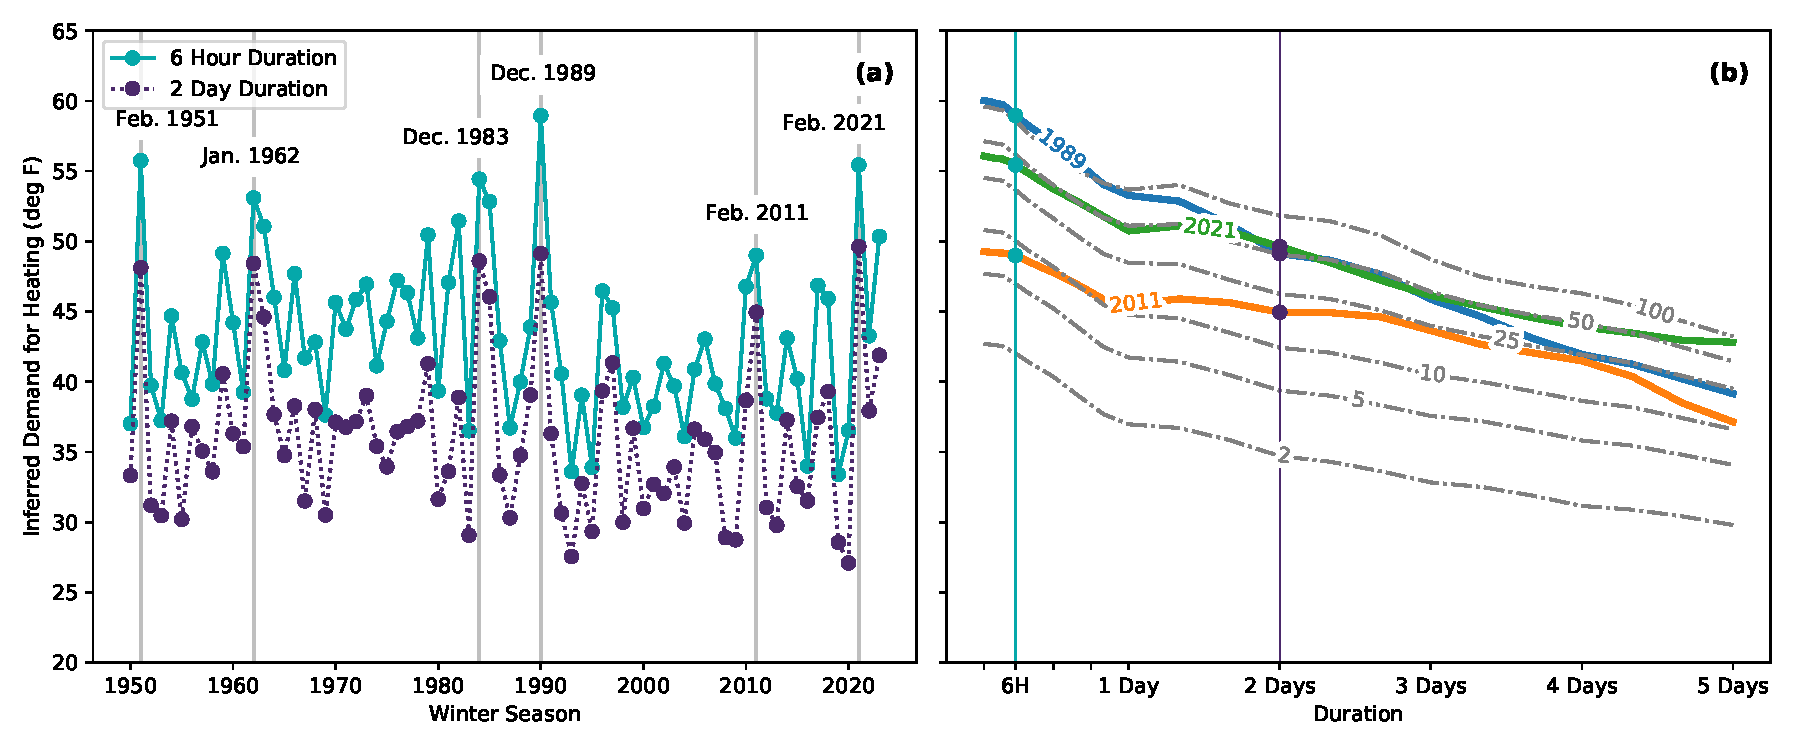
\includegraphics[width=\textwidth]{ERCOT_HDD_IDF_MLE_unweighted.pdf}
  \caption{
    As \cref{fig:idf_unweighted} but grid cells are weighted by area $A=\cos(\phi)$ where $\phi$ is latitude.
  }\label{fig:idf_unweighted}
\end{figure}

\begin{figure}
  \centering
  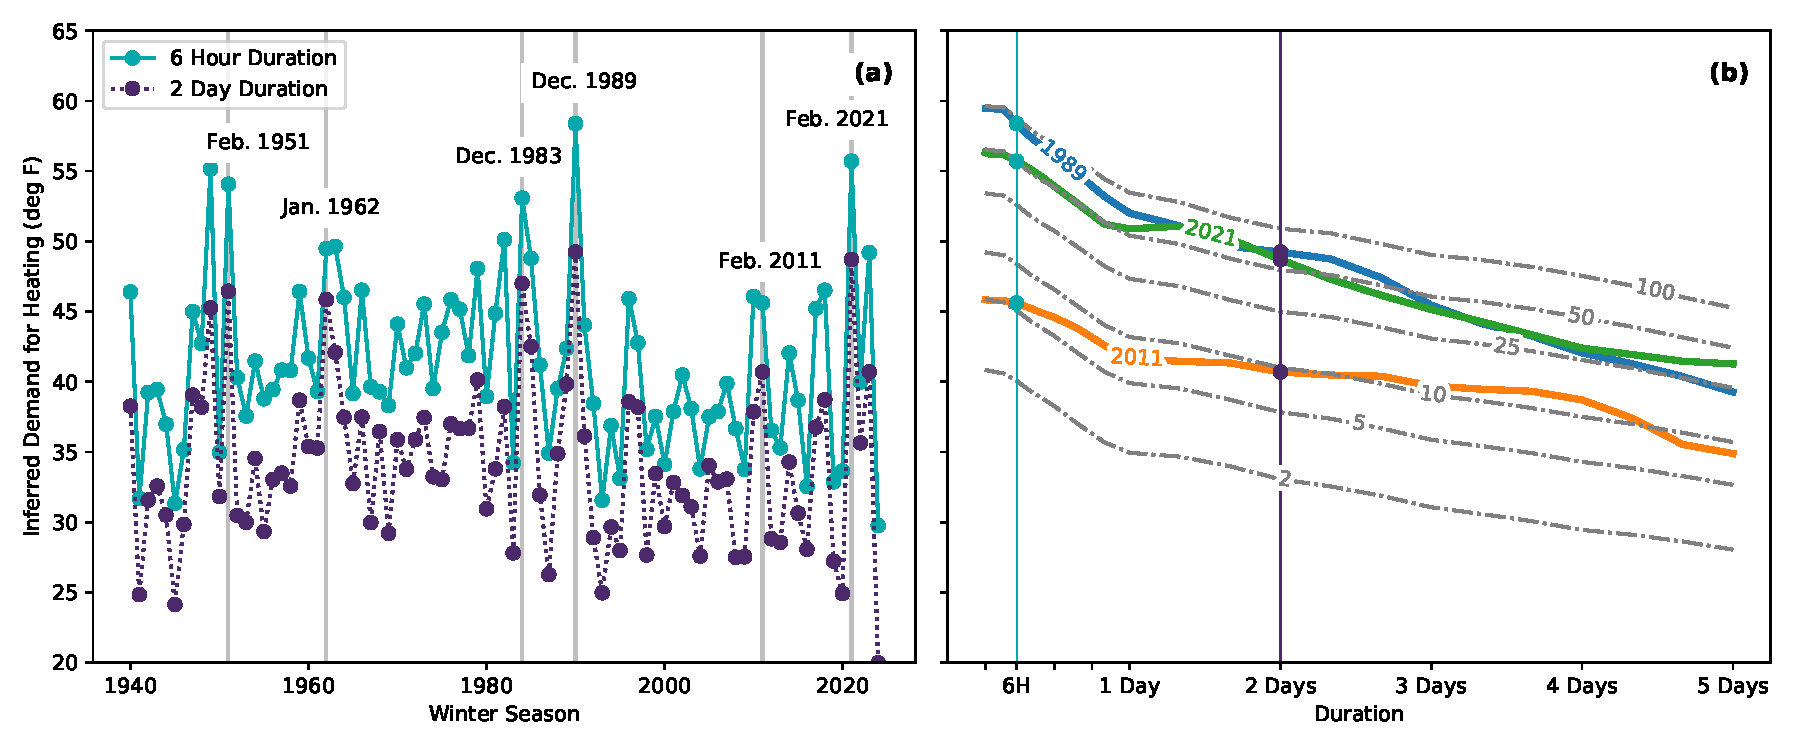
\includegraphics[width=\textwidth]{ERCOT_HDD_IDF_plotpos_popweighted.pdf}
  \caption{
    As \cref{fig:idf_unweighted} but return periods are calculated using the $L$-moments estimator.
  }\label{fig:idf_lmoments_weighted}
\end{figure}

\begin{figure}
  \centering
  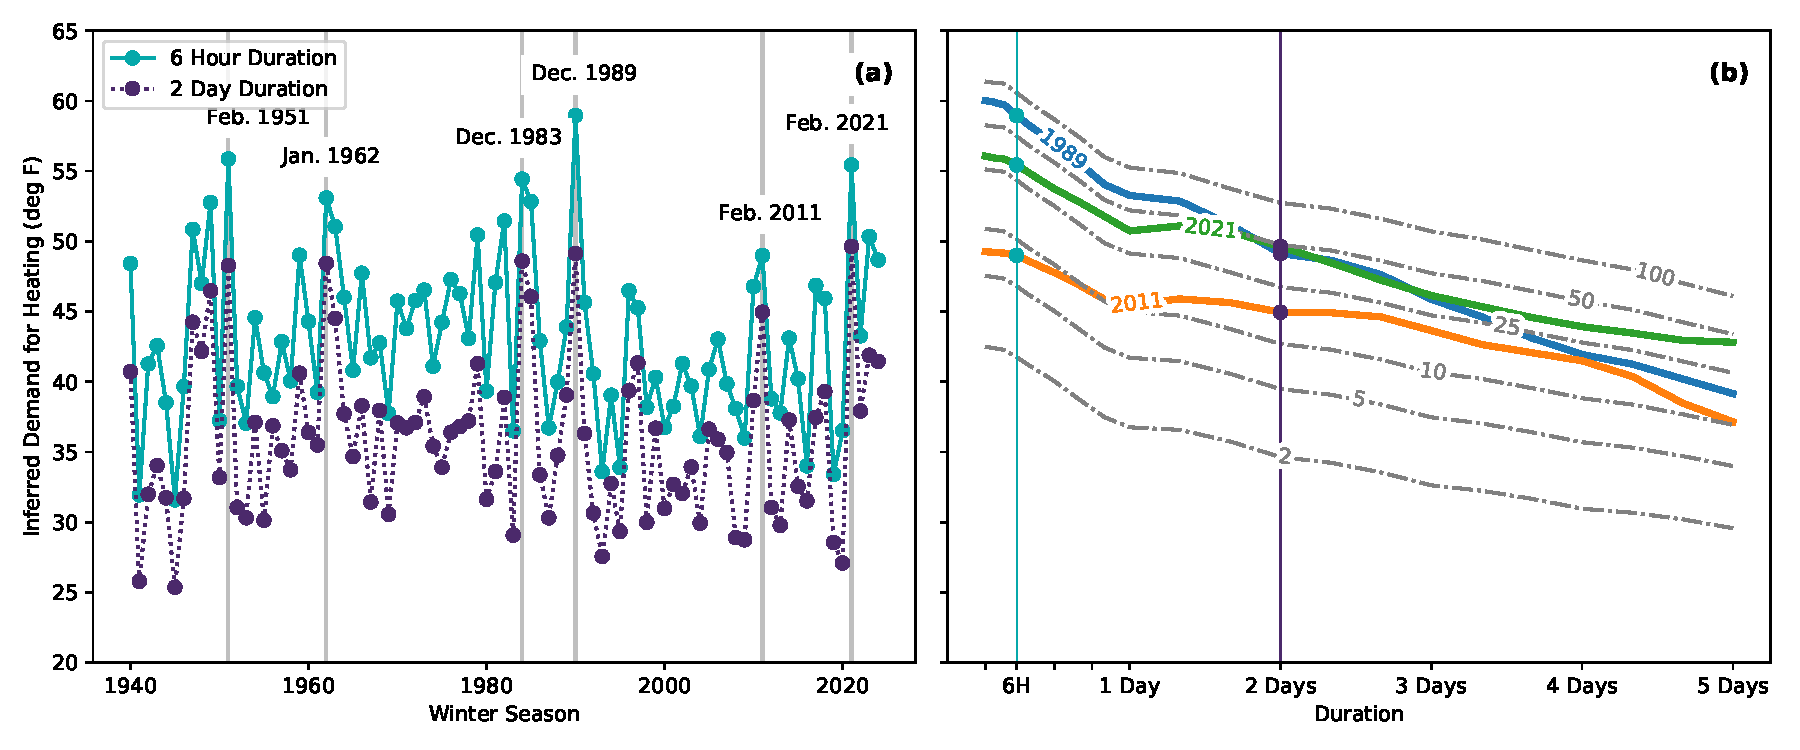
\includegraphics[width=\textwidth]{ERCOT_HDD_IDF_plotpos_unweighted.pdf}
  \caption{
    As \cref{fig:idf_unweighted} but return periods are calculated using the $L$-moments estimator.
  }\label{fig:idf_lmoments_unweighted}
\end{figure}

\begin{figure}
  \centering
  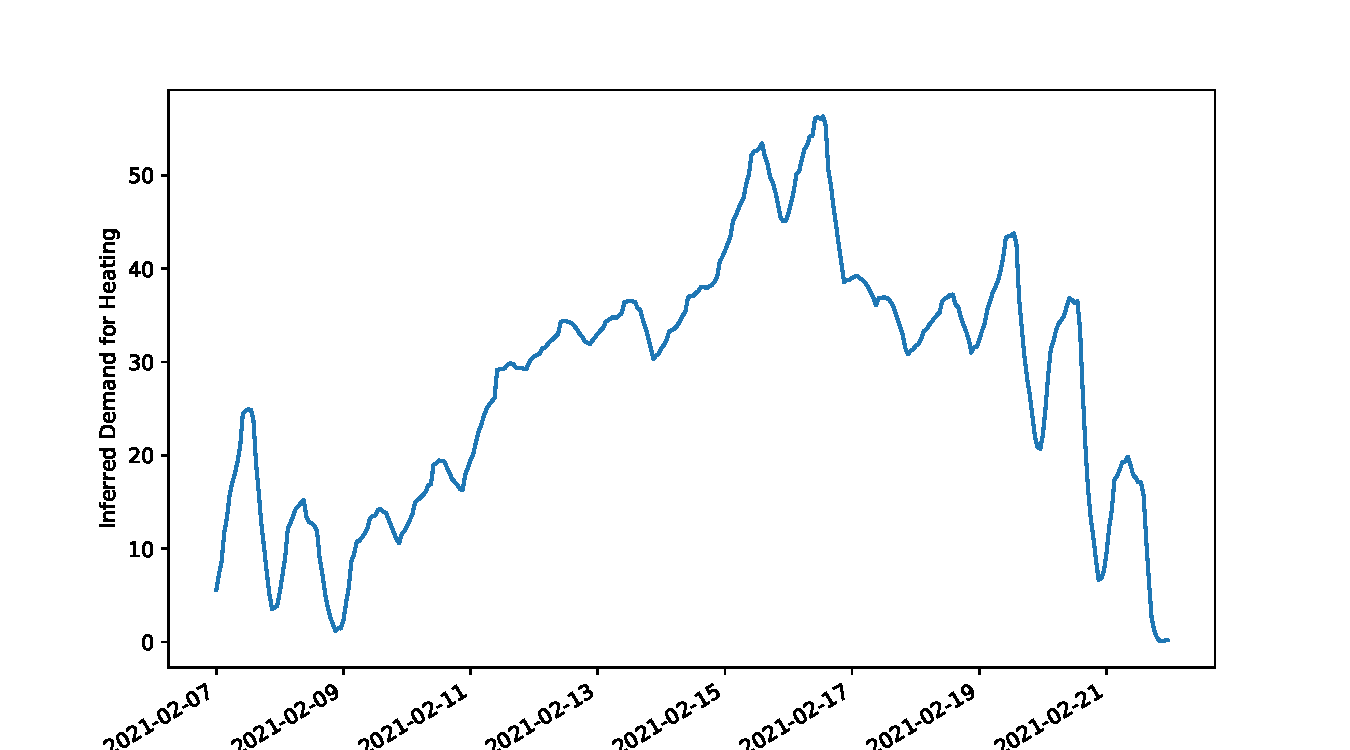
\includegraphics[width=\textwidth]{HDD_pop_weighted_ts.pdf}
  \caption{
    A time series of inferred \DIFdelbeginFL \DIFdelFL{demand for }\DIFdelendFL heating \DIFaddbeginFL \DIFaddFL{demand per capita }\DIFaddendFL over the Texas \DIFdelbeginFL \DIFdelFL{Interconnect }\DIFdelendFL \DIFaddbeginFL \DIFaddFL{Interconnection }\DIFaddendFL during the February 2021 cold snap.
  }\label{fig:hdd_ts}
  \DIFaddbeginFL \end{figure}

\begin{figure}
  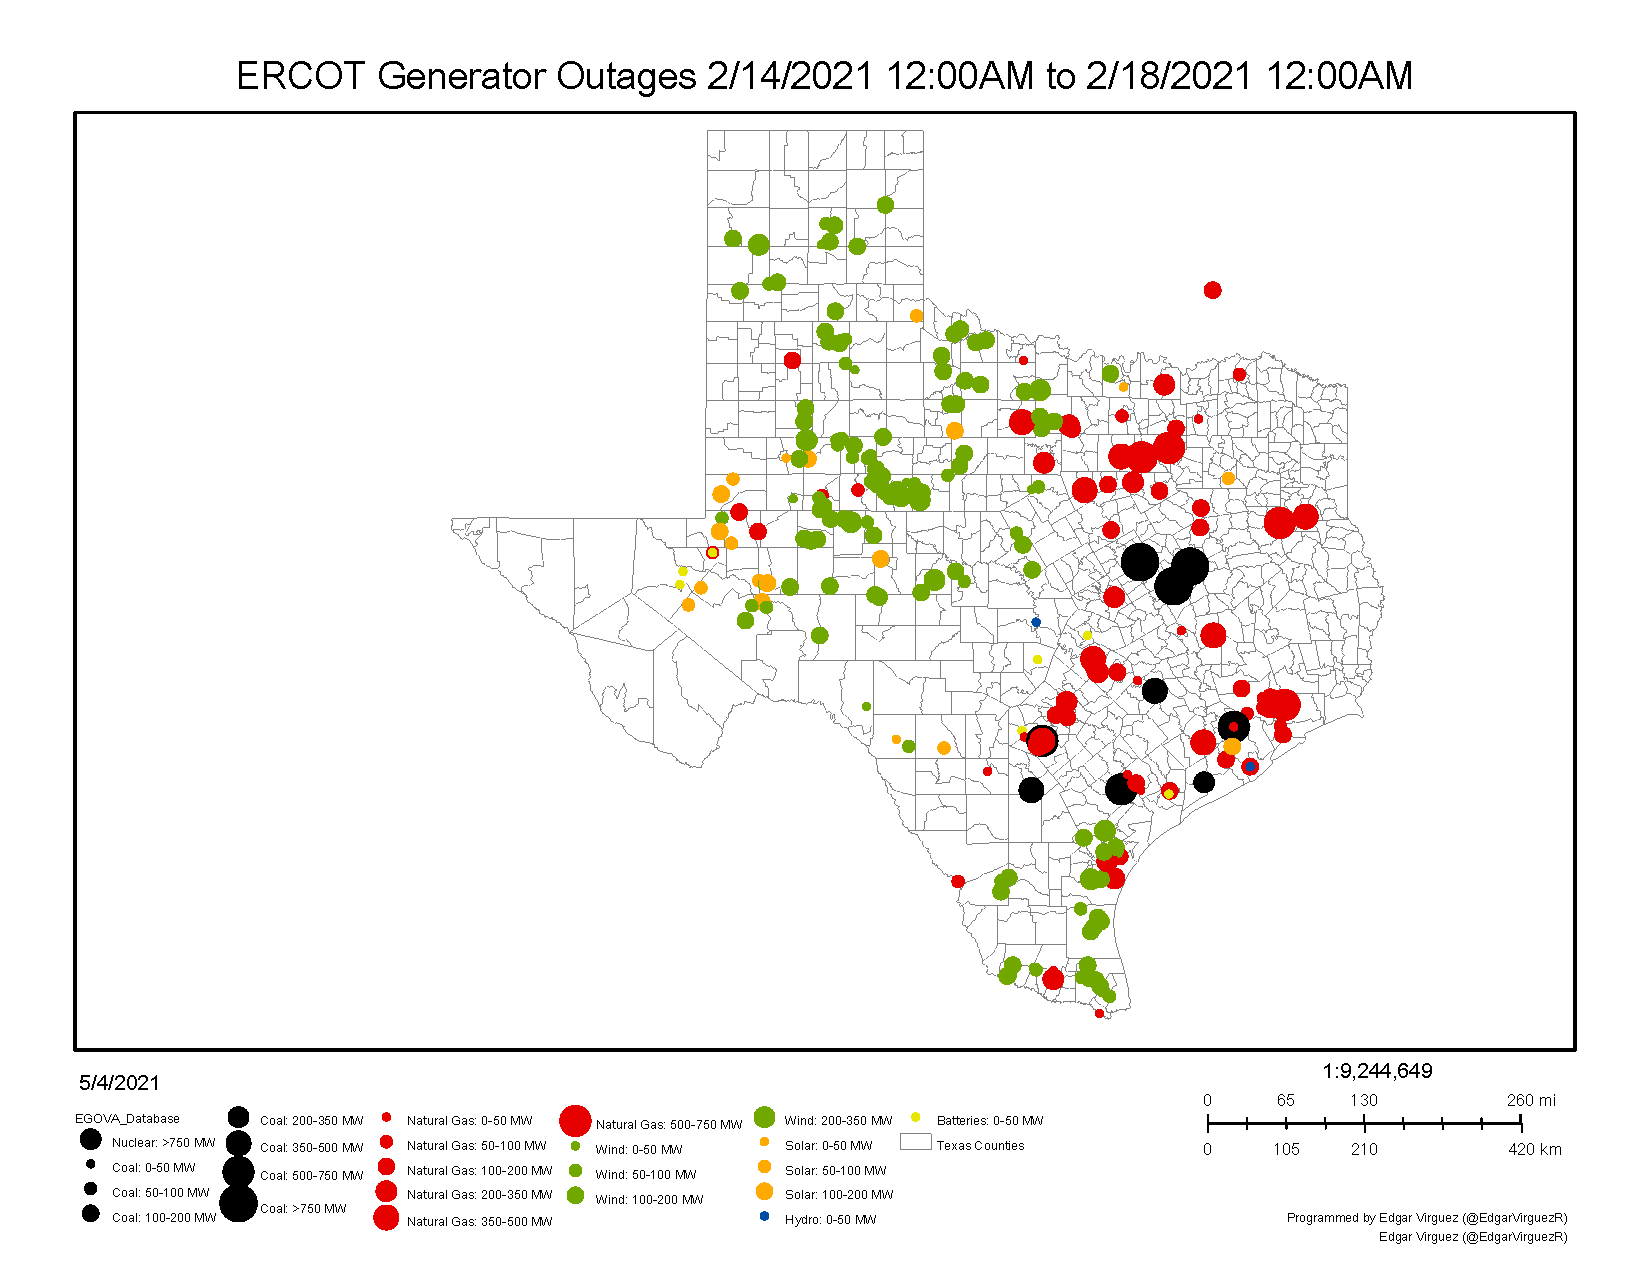
\includegraphics[width=\textwidth]{EGOVA.pdf}
  \caption{
    \DIFaddFL{ERCOT generator outages from 12:00AM on 14 February 2021 to 12:00AM on 18 February 2021.
      Map produced using ERCOT's Generator Outage/Derate Visualization App (EGOVA) available at }\url{https://bit.ly/EGOVA}\DIFaddFL{.
    }}\label{fig:egova}
  \DIFaddendFL \end{figure}

\end{document}

